\documentclass[sustainability,article,accept,moreauthors]{Definitions/mdpi}
\newif\ifmarkchanges
\ifdefined\CleanVersion\markchangesfalse\else\markchangestrue\fi
\DeclareRobustCommand{\rev}[1]{\ifmarkchanges{\hypersetup{linkcolor=blue,citecolor=blue,urlcolor=blue}\textcolor{black}{#1}}\else#1\fi}




\usepackage{amsmath}
\usepackage{booktabs}
\usepackage{array}
\usepackage{graphicx}
\usepackage{longtable}
\usepackage{enumitem}
\usepackage{pdflscape}
\setlength{\headheight}{20pt}
\addtolength{\topmargin}{-8pt}
\newcolumntype{Y}{>{\raggedright\arraybackslash}X}

\graphicspath{{figures/}}
\newcolumntype{P}[1]{>{\raggedright\arraybackslash}p{#1}}
\newcommand{\TableNote}[1]{\noindent{\footnotesize{#1}}}

\firstpage{1}
\makeatletter
\setcounter{page}{\@firstpage}
\makeatother
\pubvolume{1}
\issuenum{1}
\articlenumber{0}
\pubyear{2026}
\copyrightyear{2026}
\externaleditor{Firstname Lastname} % More than 1 editor, please add `` and '' before the last editor name
\datereceived{27 July 2026}
\daterevised{22 September 2026}
\dateaccepted{23 September 2026}
\datepublished{}

\Title{\textls[-15]{Calibrating Generative AI Use for Sustainable Higher Education: \highlighting{Cross-Sectional Evidence} %MDPI: Article title is different from the one submitted online at susy.mdpi.com. Please confirm which is correct.
 on Perceived Capability and~Dependence}}

\newcommand{\orcidauthorA}{0009-0000-9137-9965}
\newcommand{\orcidauthorB}{0009-0008-3195-5631}
\newcommand{\orcidauthorC}{0009-0005-8650-1563}

\Author{\hl{Xinchen Zhang} %MDPI: Please carefully check the accuracy of names and affiliations.
\orcidA{}, Yile Wang \orcidB{} and Chunbing Li *\orcidC{}}
\AuthorNames{Xinchen Zhang, Yile Wang and Chunbing Li}

\address[1]{%
School of Economics, Beijing Technology and Business University, Beijing 102488, China; 2401090227@st.btbu.edu.cn (X.Z.); 2401050128@st.btbu.edu.cn (Y.W.)}

\corres{\hangafter=1 \hangindent=1.05em \hspace{-0.82em}Correspondence: licb@th.btbu.edu.cn}

\abstract{Generative artificial intelligence (GenAI) can support educational work while changing how users engage in independent generation and evaluation. This study examines whether the GenAI task use frequency has different associations with perceived role-specific capability and AI dependence. A cross-sectional survey of 1105 respondents (659 students and 446~teachers) from five Beijing universities measured all focal variables by self-report. Hierarchical regressions with HC3 standard errors were complemented by formal inverted U tests, bootstrap intervals, measurement-model sensitivity analyses, and nested out-of-fold prediction. Both capability outcomes showed positive lower-range and negative upper-range slopes, with the maxima located within the observed use range and supported by observations on both sides within each literacy stratum. Between the 25th and 75th percentiles of AI literacy, the model-implied maximum shifted by 0.715 use scale units for students (95\% bootstrap CI \highlighting{[0%MDPI: Newly added 0, the following highlights are the same, please check all.
.525, 0.973])} and 0.643 units for teachers (95\% CI \highlighting{[0.450, 0.883]).} The primary literacy measure was a 12-item mean; four-dimensional and second-order CFA specifications supported its interpretation as a broad composite. Separate exploratory dimension models yielded positive literacy-by-use interactions, with the largest point estimate for critical evaluation. Dependence was positively associated with use, habit, and trust and negatively associated with literacy. The combined squared use and interaction increments for dependence were \highlighting{0.0024} and \highlighting{0.0004,} with 90\% interval upper bounds of \highlighting{0.0058} and \highlighting{0.0031,} below an exploratory \highlighting{0.01} $R^2$ benchmark. Belief-centred and trust omission specifications supported the broader reliance pattern, although trust and dependence remained conceptually close. Nonlinear ridge recovered most of the capability prediction improvement over linear ridge. The findings describe between-person associations, not individual optimal use levels or intervention effects. They motivate the evaluation of literacy-oriented task design and complementary approaches to trust calibration and habitual reliance.}

\keyword{generative artificial intelligence; sustainable higher education; SDG 4; AI literacy; perceived learning agency; teaching innovation competence; AI dependence; cognitive offloading; inverted U relationship}

\begin{document}
\hypersetup{pdfsubject={Research article -- sustainability-4495862}}

\section{Introduction}\label{sec:intro}

\textls[-15]{The sustainability of higher education depends not only on the present educational output but also on whether institutions continue to reproduce the human capabilities required for learning, judgement, and professional action. Sustainable Development Goal~4 (SDG~4) consequently extends beyond access and attainment to relevant skills, lifelong learning, education for sustainable development, and qualified teachers~\cite{unesco2023,joseph2025}. Digital technologies can support these objectives by widening access and lowering the cost of individualised assistance. Yet increased adoption is not itself evidence of educational sustainability. A technology may improve immediate task completion while displacing the cognitive activity through which transferable knowledge, judgement, and professional agency are renewed~\cite{bulathwela2024,su2026}.}

Generative artificial intelligence (GenAI) makes this distinction especially consequential. Students use GenAI for explanation, drafting, translation, programming, and assessment preparation; teachers use it for lesson design, feedback, resource development, and administrative work~\cite{chiu2024}. Meta-analyses report positive average effects of GenAI-supported interventions on academic performance~\cite{sunzhou2024,gu2025}. These gains do not establish whether more frequent use is uniformly associated with stronger independent capabilities. Guided systems may scaffold problem-solving, whereas unrestricted assistance can improve assisted performance without producing equivalent gains after the support is removed~\cite{bastani2025,fan2025}. Sustainable integration therefore requires attention to both the immediate value of assistance and the human work that assistance replaces.

Cognitive offloading research provides a mechanism for both possibilities. External support can release working memory resources and permit attention to shift towards higher-order activity~\cite{sweller2019}. The same support can replace retrieval, generation, error monitoring, and metacognitive regulation, which are central to durable learning and judgement~\cite{risko2016,bjork2011,sparrow2011}. At low or moderate use, examples, feedback, and inexpensive iteration may operate primarily as scaffolds. At higher use, the marginal benefit of scaffolding may diminish while substitution increases. This combination predicts a concave association rather than a constant linear effect~\cite{pierce2013,haans2016,zhao2025}.

Capability and dependence must nevertheless be distinguished. In this study, perceived role-specific capability refers to students' perceived learning agency and teachers' self-reported teaching innovation competence. AI dependence refers to self-reported cognitive and behavioural reliance on AI-supported task execution~\cite{morales2024,du2026,kalimira2026}. Trust can make delegation acceptable under uncertainty~\cite{lee2004,hoff2015}, while repeated behaviour in stable contexts can become habitual and progressively less deliberative~\cite{limayem2007,woodneal2007}. A respondent may therefore report both high capability and high dependence. Treating the outcomes as opposite ends of one scale would conceal this possibility.

AI literacy may alter both pathways. Awareness, practical use, critical evaluation, and ethical judgement help users to identify task boundaries, verify outputs, recognise uncertainty, and retain responsibility for consequential decisions~\cite{long2020,wang2023}. Existing studies mainly treat literacy as a direct resource associated with self-efficacy, output quality, innovative behaviour, or lower dependence~\cite{becirovic2025,zhang2025,zi2026}. Selective offloading theory implies a stronger boundary condition claim: literacy may widen the range over which use accompanies capability by improving the quality of delegation, even if it does not eliminate habit formation~\cite{tankelevitch2024,bucinca2021}.

Most evidence concerns students. Teachers require parallel analysis because their use affects lesson design, feedback, assessment, and the learning environments experienced by multiple cohorts~\cite{zhaiTeacher2025}. The present study therefore estimates separate student and teacher models while retaining role-specific outcomes.

\textls[-25]{Before reviewing the detailed theory, the study is organised around four research~questions:}

\begin{enumerate}[label=\textbf{\hl{RQ}%MDPI: Please confirm if the bold formatting is necessary; if not, please remove it. The following highlights are the same.
\arabic*.},leftmargin=3.4em,labelwidth=2.75em,labelsep=.55em]
\item What functional form characterises the cross-sectional association between the GenAI task use frequency and perceived role-specific capability?
\item Does AI literacy, considered both globally and by dimension, shift the location of the model-implied capability maximum?
\item Do use, trust, habit, literacy, and perceived risk relate to AI dependence through a predominantly additive structure that is distinct from the capability pathway?
\item To what extent does the dual-path structure converge across student and teacher cohorts despite role-specific outcome measures?
\end{enumerate}

The theoretical review below is organised around these questions and develops four hypotheses, with the quantitative assessment of H4 treated as exploratory. The contribution is a dual-outcome model of the individual-level micro-foundations of sustainable GenAI integration: the capacity to renew perceived role-specific capability while keeping reliance patterns governable and reversible~\cite{chen2026}.

\section{Theoretical Background and Hypotheses}\label{sec:theory}

\subsection{Framework, Assumptions, and Level of Analysis}\label{sec:framework}

The framework integrates cognitive offloading, the
scaffolding--substitution distinction, trust and habit accounts of reliance, and a sustainability perspective. The framework rests on five assumptions about assistance, perceived capability, literacy, reliance, and institutional sustainability.
\begin{enumerate}
\item \textbf{\hl{Assistance can scaffold or substitute.}} GenAI support can complement users' own generation and evaluation, but it can also replace these processes. The balance can change with the use frequency.
\item \textbf{\hl{Perceived capability and dependence are distinct outcomes.}} Capability concerns respondents' appraisal of their learning or professional agency; dependence concerns reliance tendencies. They may move together or diverge.
\item \textbf{\hl{AI literacy is a supervisory boundary condition.}} Literacy supports task selection, verification, and accountability and should therefore affect where the use--capability association changes direction.
\item \textbf{\hl{Trust and habit sustain reliance.}} Trust reduces the perceived uncertainty of delegation, while habit links repeated delegation to stable cues. Neither mechanism requires an interior maximum.
\item \textbf{\hl{Institutional sustainability is an aggregation proposition.}} The constructs are measured at the individual level. Their relevance to sustainable higher education rests on the proposition that repeated individual patterns accumulate into an institution's capacity to regenerate human judgement and maintain reversible modes of technology use. This temporal aggregation is theorised here but not directly observed in the cross-sectional design.
\end{enumerate}

For the present study, \emph{\hl{capability stock}%MDPI: Please confirm if the italics are necessary; if not, please remove them. The following highlights are the same.
}, \emph{\hl{reversibility}}, and \emph{\hl{reliance lock-in}} are therefore theoretical propositions rather than directly measured institutional constructs. They distinguish sustainability from the narrower question of whether any single act of GenAI use is responsible or effective. Sustainability concerns whether the human capability base on which future teaching and learning depend is renewed over time and whether reliance remains open to deliberate interruption. The empirical study tests individual-level patterns that constitute possible micro-foundations of these institutional processes.


\subsection{Use Frequency and Perceived Educational Capability}

At low to moderate frequencies, GenAI can provide examples, feedback, alternative explanations, and inexpensive opportunities for iteration{~\cite{chiu2024}}. When users retain responsibility for problem formulation, evaluation, and revision, these affordances can reduce extraneous loads and support self-regulated learning or instructional experimentation{~\cite{wood1976,sweller2019}}. Positive average effects in intervention research are consistent with this scaffolding mechanism~\cite{sunzhou2024,gu2025}. {A cross-context example comes from heritage tourism VR, where affective responses and perceived value are linked to reuse intention~\highlighting{\cite{jiang2026information}.} %MDPI: We revised the order of the reference citations. Please confirm.
 This illustrates why the experiential appeal of continued technology use should be distinguished from the cognitive processes that support educational capability.}


\begin{table}[H]
\caption{\hl{Theoretical} %MDPI: 1. Please cite this table in the text and ensure that the first citation of each table appears in numerical order. 2. To reduce blank space on the page, we have moved Table 1 here. Please confirm.
 assumptions and their empirical representation.}
\label{tab:framework}
\small
\begin{adjustwidth}{-\extralength}{0cm}
\begin{tabularx}{\fulllength}{P{4cm}P{4.2cm}P{4.2cm}P{4cm}}
\toprule
\textbf{Theoretical Proposition} & \textbf{Empirical Representation} & \textbf{Focal Prediction} & \textbf{Status in This Design}\\
\midrule
Scaffolding and substitution coexist & Five-item GenAI task use frequency index and its squared term & Interior maximum in perceived capability & Tested as a cross-sectional functional form\\
Literacy supports selective offloading & Observed 12-item literacy mean and four component dimensions & Positive capability association and rightward shift of maximum & Tested as main effect and moderation\\
Trust and habit sustain reliance & Trust, habit, and perceived risk scales & Predominantly additive dependence pathway & Tested with regression and sensitivity models\\
Capability renewal and reliance reversibility support sustainability & Student and teacher role-specific outcomes & Parallel dual-path structure across roles & Individual-level micro-foundation; institutional process not directly measured\\
\bottomrule
\end{tabularx}
\end{adjustwidth}
\end{table}

The same delegation can become substitutive as use becomes routine. Durable capability depends on retrieval, generation, error detection, and desirable difficulty~\cite{bjork2011}. When GenAI repeatedly supplies both an answer and an apparent reasoning path, users may complete more tasks while engaging less with the processes that build transferable knowledge and judgement. Evidence demonstrating that assisted performance can exceed subsequent independent performance illustrates this distinction~\cite{bastani2025,fan2025}. Survey findings connecting intensive use with procrastination, memory concerns, and lower performance are directionally consistent, although they do not establish temporal order~\cite{zhaiReview2024,abbas2024}.

The too-much-of-a-good-thing framework integrates the two mechanisms. If the marginal benefit of scaffolding declines while the marginal cost of substitution rises, the association reaches an interior maximum~\cite{pierce2013,haans2016}. Because the outcomes are self-reported, the empirical claim concerns perceived learning agency and self-reported teaching innovation competence rather than independently tested post-withdrawal performance. A second boundary should be stated at the outset rather than deferred to the Limitations. The use measure indexes how often GenAI is employed across task types, not how deeply any task is delegated; the scaffolding--substitution mechanism is therefore inferred from the shape of the association rather than observed directly (Section~\ref{sec:measures}).

\begin{Hypothesis}
The GenAI task use frequency has an inverted U association with perceived role-specific educational capability, i.e., perceived learning agency among students and self-reported teaching innovation competence among teachers.
\end{Hypothesis}

\subsection{AI Literacy and the Location of the Model-Implied Maximum}

AI literacy comprises awareness, practical use, critical evaluation, and ethical judgement~\cite{wang2023}. These dimensions function as supervisory competencies: they help users to decide what to delegate, assess whether an output is adequate, detect uncertainty, and retain accountability. In metacognitive terms, literacy supports selective rather than indiscriminate offloading~\cite{tankelevitch2024}. Cognitive forcing functions that require reflection on AI advice provide related evidence that active evaluation can reduce overreliance~\cite{bucinca2021}.

At a given use frequency, a more literate respondent should therefore be more likely to employ GenAI as a complement than as a substitute. The model-implied point at which the capability association turns downward should occur at a higher use level. This remains a bounded claim: literacy may widen the productive range without making unlimited delegation beneficial.

\begin{Hypothesis}
(a) AI literacy is positively associated with perceived role-specific capability; (b) AI literacy shifts the model-implied capability maximum towards a higher level of GenAI task use~frequency.
\end{Hypothesis}

\subsection{Trust, Habit, Risk, and AI Dependence}

Dependence is expected to follow a different process. Trust is the belief that makes reliance acceptable under uncertainty, and inappropriate trust can create measurable costs of overreliance~\cite{lee2004,klingbeil2024}. Habit develops when repeated behaviour becomes linked to stable cues and increasingly automatic~\cite{woodneal2007}. In information systems continuance, habit can sustain behaviour even as conscious intention becomes less predictive~\cite{limayem2007}. The I-PACE framework similarly proposes that repeatedly rewarded interactions strengthen links among situational cues, appraisal, and automatic execution~\cite{brand2016}.

Unlike the capability pathway, trust--habit accumulation has no theoretical requirement for an interior maximum. Dependence may decelerate near a scale ceiling, but it should not decline merely because use becomes more frequent. Perceived risk should provide a countervailing appraisal by increasing scrutiny. AI literacy should lower dependence by supporting informed control, although literacy need not prevent repeated delegation from becoming automatic.

\begin{Hypothesis}
The GenAI task use frequency, trust, and habit are positively associated with AI dependence, whereas AI literacy and perceived risk are negatively associated with dependence.
\end{Hypothesis}

Nonlinear and interaction terms are therefore expected to add little incremental explanatory value to the dependence models. The theoretical expectation concerns the relative importance of these terms, rather than the absence of any curvature. The quantitative assessment uses an exploratory benchmark of  0.01 additional explained variance (one percentage point of $R^2$). This benchmark is exploratory rather than a preregistered equivalence margin~\cite{lakens2017}.

\begin{Hypothesis}
Compared with the capability pathway, the dependence pathway is predominantly additive: squared use and literacy-by-use terms contribute relatively little additional explanatory value, and no capability-like interior maximum appears within the observed range.
\end{Hypothesis}

\subsection{Cross-Role Structural Convergence}

Students and teachers delegate different tasks, but the cognitive structure of delegation is comparable. Students may delegate explanation, drafting, and problem-solving; teachers may delegate lesson planning, feedback, and resource design. AI literacy and pedagogical knowledge shape teachers' integration decisions~\cite{alabdullatif2024,ning2024}, but professional experience does not necessarily prevent habitual reliance.
RQ4 therefore asks whether the sign and functional-form pattern converges across cohorts. It does not assert scale equivalence or identical coefficient magnitudes because the capability outcomes are role-specific.

H1--H3 state the directional expectations motivating the primary regressions. H4's quantitative benchmark, RQ4, the dimension-level literacy models, the decomposition of the use index, and unanticipated associations are treated as exploratory or post hoc and are labelled accordingly. No analysis is represented as preregistered.
Figure~\ref{fig:model} summarises the framework and labels the tested paths explicitly.

\begin{figure}[H]
\centering
\begin{adjustwidth}{-\extralength}{0cm}
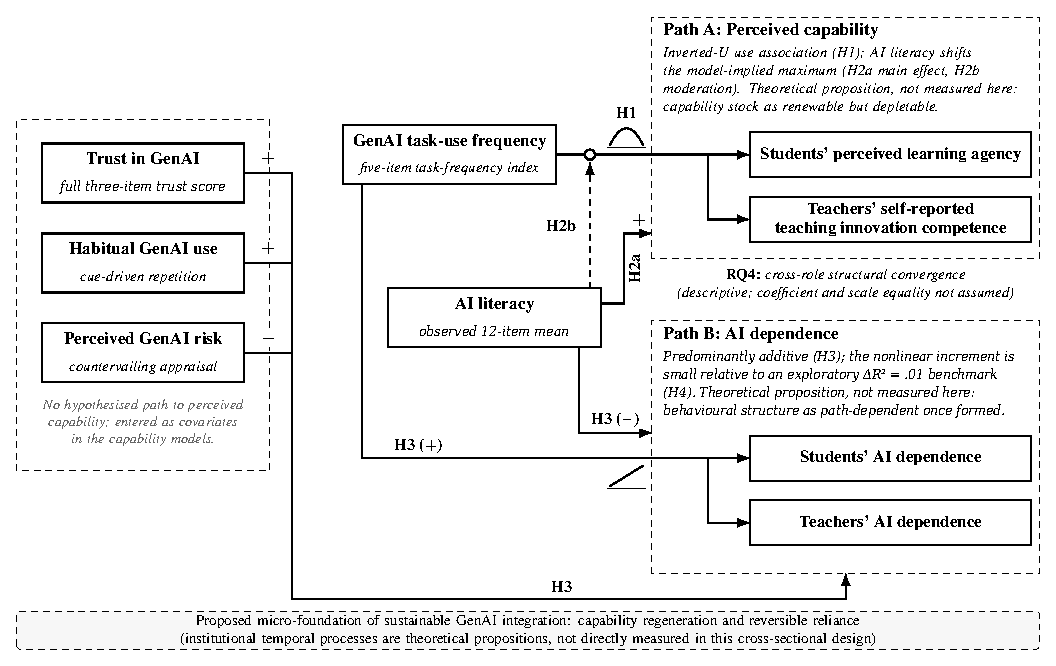
\includegraphics[width=\fulllength]{fig_conceptual_model_clean.pdf}
\end{adjustwidth}
\caption{Conceptual model. H1 concerns the inverted U use--capability association; H2 concerns the positive literacy association and rightward shift of the model-implied maximum; H3 concerns the additive predictors of AI dependence; and H4 compares the nonlinear dependence increment with an exploratory \hl{$\Delta R^2=0.01$} benchmark. RQ4 evaluates cross-role structural convergence without assuming coefficient or scale equality. Primary regressions use the observed 12-item literacy mean and the full three-item trust score. The second-order literacy specification and the two-item trust score are measurement and sensitivity models, respectively. The sustainability band denotes an institutional-level theoretical proposition whose temporal properties are not directly measured in the cross-sectional survey.}
\label{fig:model}
\end{figure}

\section{Materials and Methods}

\subsection{Design, Participants, Ethics, and Procedure}\label{sec:design}

The study used a cross-sectional, parallel-instrument survey design. Ethical approval was granted by the Science Research Ethics Committee of Beijing Technology and Business University on 1 September 2025 (protocol 2025-(70)), before data collection from October through December 2025. Participation was voluntary and anonymous. Before accessing the questionnaire, respondents received information about the study purpose, procedures, voluntariness, withdrawal, anonymity, and data handling and provided affirmative electronic consent. All participants were at least 18 years old.

An institution-based convenience sample was recruited from enrolled students and teaching staff at five universities in Beijing. To preserve institutional anonymity, the institutions are described as one comprehensive research university, one teacher education university, one science and engineering university, one business and economics university, and one application-oriented multidisciplinary university. Recruitment used institutional mailing lists, course and staff communication groups, and QR code links distributed by local coordinators. Affiliation was retained as a five-category code for clustering sensitivity analyses. The sample is not claimed to be probabilistically representative of Chinese higher education. Institution-level invitation counts were not retained, so a population response rate cannot be calculated. Future waves will preserve the per-institution invitation registers and reconcile them against the completed questionnaires. During the collection window, none of the five institutions prohibited GenAI use, and guidance was left largely to individual instructors. No institution provided a universal licence for paid tools, so access relied mainly on publicly available Chinese-language chatbots, under the same conditions for students and teachers. These shared access conditions plausibly shape both the reported use frequency and the meaning of dependence, and cross-context replication should record them systematically.

The fieldwork protocol contained two embedded instructed-response attention checks. The first requested the selection of ``Agree'' and the second requested the selection of ``Strongly disagree''. Respondents were excluded if either item was answered incorrectly, if the total completion time was below 180 s, or if duplicate browser and long string checks indicated a patterned or duplicate response. The rules were fixed before the inspection of the focal outcomes. The questionnaire used required responses for core items, so no core values were imputed.
A total of 1196 questionnaires were returned. Ninety-one were excluded under the quality screening protocol, leaving 1105 respondents: 659 students and 446 teachers. Table~\ref{tab:sample} makes the cohort-specific analytical flow explicit. The 92.4\% retention proportion refers to returned questionnaires after quality screening and is not a response rate.

\begin{table}[H]
\caption{Cohort-specific analytical flow and institutional composition.}
\label{tab:sample}
\small
\begin{adjustwidth}{-\extralength}{0cm}
\begin{tabularx}{\fulllength}{lCCC}
\toprule
\textbf{Stage or Characteristic} & \textbf{Students} & \textbf{Teachers} & \textbf{Total}\\
\midrule
Returned questionnaires &
713 & 483 & 1196\\
Failed at least one attention check &
30 & 20 & 50\\
Below completion time threshold & 17 & 12 & 29\\
Patterned or duplicate response & 7 & 5 & 12\\
Final analytical sample & 659 & 446 & 1105\\
\midrule
Institution A & 145 & 89 & 234\\
Institution B & 128 & 94 & 222\\
Institution C & 132 & 82 & 214\\
Institution D & 126 & 91 & 217\\
Institution E & 128 & 90 & 218\\
\midrule
Age, $M$ ($SD$); range & 20.61 (2.63); 18--29 & 42.59 (8.78); 26--65 & ---\\
Teaching experience, $M$ ($SD$); range & --- & 14.24 (7.61); 0--36
& ---\\
Disciplinary categories & 7 & 7
&
---\\
Missing core responses after screening & 0 & 0 & 0\\
\bottomrule
\end{tabularx}
\end{adjustwidth}
\TableNote{Notes: Exclusion reasons are mutually exclusive primary reasons assigned in the order shown. Institution labels are anonymised.}
\end{table}

\subsection{Instrument Development, Translation, and Adaptation}\label{sec:instrumentdev}

The questionnaire was administered in Chinese. English-language source items were independently translated by two bilingual researchers, reconciled through discussion, and back-translated by a third bilingual researcher who had not seen the original wording. Discrepancies were resolved by comparing semantic content rather than the literal word order. The research team then reviewed construct coverage, role equivalence, and clarity. A pilot with 48 respondents (30 students and 18 teachers) assessed the completion time, comprehension, and item ambiguity; minor wording changes were made to four role-specific items without changing their intended constructs. The student and teacher versions retained parallel stems where possible and changed only the task referent, such as learning tasks versus teaching design tasks. Appendix~\ref{app:instrument} provides an English item map, the literature and wording notes for each construct, scoring rules, and standardised loadings (Tables~\ref{tab:items} and~\ref{tab:background}). The English wording is the reconciled back-translation, rather than the original Chinese administration form.

\subsection{Measures}\label{sec:measures}

Except for the task use frequency index, all focal constructs used seven-point agreement scales (1 = strongly disagree, 7 = strongly agree). GenAI task use frequency used the following categories: 1 = never; 2 = less than once a month; 3 = one to three times a month; 4~=~about once a week; 5 = several times a week; 6 = about once a day; and 7~=~multiple times per day. The single overall frequency control used the same categories. These ordered codes were averaged as a task frequency index rather than converted into estimated daily event counts. Construct scores were calculated as unweighted item means, with no reverse-coded items. The five-item task use score is distinct from the single overall frequency control. All distributional summaries, spline knots, and support counts use this same five-item score within the corresponding analytical cohort.

AI literacy was measured with 12 items representing awareness, practical use, critical evaluation, and ethical judgement, following the Artificial Intelligence Literacy Scale~\cite{wang2023}. Rather than treating the 12 items as a single first-order factor by default, the analysis compared a one-factor model, four correlated first-order dimensions, and a second-order literacy model. The primary regressions used the unweighted mean of the 12 items. Because each dimension contained three items, this was also the equally weighted mean of the four dimension scores. The CFA comparisons evaluate the structural rationale for this broad summary; they do not convert the arithmetic mean into a latent factor score. Separate dimension models and a CFA factor score sensitivity analysis examine dependence on the scoring approach.

The GenAI task use frequency was measured with five parallel task frequency items tailored to learning activities for students and teaching activities for teachers. The index measured the frequency across task types, not the proportion of work delegated or the consequences of delegation.

For the decomposition, one model substitutes the mean of USE1--USE3 for overall task use, and a separate model substitutes the mean of USE4--USE5. Each contains the substituted use score, its square, the literacy main effect, and the literacy-by-use interaction with the original controls; the two indices are not entered jointly. An exploratory decomposition distinguishes three support-oriented items from two more substitution-proximal items; because this classification was not prespecified and could not recover the delegation depth directly, it is reported as sensitivity evidence rather than a new confirmatory measure.

Trust in GenAI was represented by three items grounded in the trust-in-automation tradition~\cite{lee2004,hoff2015}; habitual GenAI use was represented by three items based on UTAUT2 and continuance research~\cite{venkatesh2012,limayem2007}; and perceived GenAI risk was represented by three items assessing errors, inappropriate reliance, and adverse consequences.
Student-perceived learning agency comprised seven items addressing goal-setting, effort regulation, choice, and purposeful learning~\cite{bandura2001,xia2026}. Teacher self-reported teaching innovation competence comprised six items addressing AI-supported pedagogical design, adaptation, and instructional innovation~\cite{mishra2023,zhaiTeacher2025}. Student AI dependence used eight items aligned with the validated dependence-on-AI construct~\cite{morales2024}; teacher AI dependence comprised five teaching-context items covering difficulty initiating tasks without AI, disruption when AI is unavailable, avoidable reliance, preference for AI suggestions, and discomfort without access. These reliance tendencies are discussed in the related teacher dependence literature~\cite{du2026}. These outcomes measure self-appraisal and reliance tendencies rather than retained performance after AI withdrawal.

The expanded specification included performance expectancy, effort expectancy, social influence, facilitating conditions, educational equity, lifelong learning orientation, demographics, study or professional background, AI tenure, and overall AI use frequency. The reliable-core specification retained the focal constructs, demographics, background variables, AI tenure, and overall frequency but excluded ancillary short scales whose reliability was below  0.70 in either cohort. Table~\ref{tab:controls} reports every ancillary control with its measurement, coding, and cohort-specific reliability; the complete side-by-side coefficient set for the expanded and reliable-core specifications is given in Appendix~\ref{app:coeffs}. Gender and discipline enter as indicator sets, with man and humanities/social sciences as the reference categories. Student models use age and study year order; teacher models use teaching experience and academic rank order. AI tenure is coded as 0--5 from never to more than 24 months, and the overall frequency retains its 1--7 code. Ordered background codes enter linearly; their coefficients describe a one-category change, not a fixed duration. Age and teaching experience are centred within the cohort. The complete-case analytical cohort is fixed across the inferential specifications; the preprocessing imputation rule in Section~\ref{sec:predictionmethods} applies only to predictor processing within the prediction pipeline.

\begin{table}[H]
\caption{Measurement, coding, and inclusion of ancillary controls.}
\label{tab:controls}
\small

\begin{tabularx}{\textwidth}{YYcccc}
\toprule
\textbf{Control} & \textbf{Items/Coding} & \boldmath{$\alpha_S$} & \boldmath{$\alpha_T$} & \textbf{Expanded} & \textbf{Reliable Core}\\
\midrule
Performance expectancy & 3-item mean & \hl{0}.681 & \hl{0}.663 & Yes & No\\
Effort expectancy & 3-item mean & \hl{0}.652 & \hl{0}.618 & Yes & No\\
Social influence & 3-item mean & \hl{0}.667 & \hl{0}.641 & Yes & No\\
Facilitating conditions & 3-item mean & \hl{0}.691 & \hl{0}.679 & Yes & No\\
Educational equity & 3-item mean & \hl{0}.644 & \hl{0}.626 & Yes & No\\
Lifelong learning orientation & 3-item mean & \hl{0}.676 & \hl{0}.659 & Yes & No\\
Gender & Indicator set & --- & --- & Yes & Yes\\
Age/experience & Centred continuous & --- & --- & Yes & Yes\\
Study year/academic rank & Role-specific background covariate & --- & --- & Yes & Yes\\
Discipline & Seven-category indicators & --- & --- & Yes & Yes\\
AI tenure & Ordered duration category & --- & --- & Yes & Yes\\
Overall AI use frequency & Seven-point frequency & --- & --- & Yes & Yes\\
Institution & Five-category indicators (sensitivity models) & --- & --- & Sensitivity & Sensitivity\\
\bottomrule
\end{tabularx}
\TableNote{Notes: The six ancillary scale scores are excluded from the reliable-core specification because $\alpha<0.70$ in at least one cohort. All demographics, discipline indicators, AI tenure, and overall use frequency remain in both~specifications.}
\end{table}
\subsection{Measurement Models and Discriminant Validity}\label{sec:measurement}

\textls[-25]{Internal consistency was assessed with Cronbach's $\alpha$, McDonald's $\omega$, and composite reliability (CR). Convergent validity was assessed with the average variance extracted (AVE), interpreted at the relevant measurement level~\cite{fornell1981}. Internal consistency and convergent validity address different properties: a high $\alpha$ or CR does not by itself resolve AVE below \hl{0}.50.}

Model-derived indices and item loadings share the same saved fit for each reported specification. With completely standardised loadings $\lambda_j$ and residual variances $\theta_j$, AVE is $\sum_j\lambda_j^2/(\sum_j\lambda_j^2+\sum_j\theta_j)$, and CR is $(\sum_j\lambda_j)^2/[(\sum_j\lambda_j)^2+\sum_j\theta_j]$. The total omega is calculated for the raw, unit-weighted item composite using the model-implied common and total covariance matrices. CR therefore refers to standardised indicators, whereas omega refers to the raw-score composite. The hierarchical omega isolates the second-order factor contribution to the 12-item score. Numerical summaries are exported at full precision before rounding for presentation. Separate covariance-based confirmatory factor analyses (CFAs) were estimated for students and teachers. In the full focal measurement model, the 12~AI literacy indicators were represented by four correlated first-order dimensions alongside six additional role-specific factors: task use frequency, trust, habit, perceived risk, perceived capability, and dependence. A companion full model represents the four literacy dimensions through a second-order factor. This factor covaries freely with each of the six other factors, which also covary freely with one another. The residuals of the four first-order literacy dimensions are mutually uncorrelated and have zero covariance with the six other factors. In this specification, any association between a literacy dimension and another factor is therefore carried by the common literacy factor, rather than estimated directly. Thus, the full-model fit statistics distinguish the correlated first-order structure from the more restrictive second-order structure. The isolated one-factor, correlated four-factor, and second-order literacy specifications were also compared directly. A supplementary multi-group assessment represents the five parallel predictor constructs by eight first-order factors: four literacy dimensions, task use frequency, trust, habit, and perceived risk. It uses the same 26 predictor indicators in both cohorts. Configural, metric, and scalar models successively impose the same loading pattern, equal corresponding loadings, and equal corresponding intercepts, with latent means freed in the teacher group at the scalar step. Factor variances, covariances, and item residual variances remain group-specific. Changes in CFI and RMSEA describe the impacts of these constraints~\cite{putnick2016}. This assessment does not establish measurement equivalence for the different student and teacher capability outcomes, which are analysed and interpreted separately.

The CFA implementation uses maximum likelihood, treating the seven-point item responses as continuous indicators and freely estimating item intercepts. The focal and literacy models fix one marker loading per factor to one; cross-loadings and item-residual covariances are zero. The isolated trust--dependence comparisons instead fix the latent variances to one and free all item loadings, so their covariance constraint directly represents a correlation. This change in scale leaves the model degrees of freedom unchanged. The student and teacher focal models contain 41 and 37 indicators, respectively. For a correlated $q$-factor model with $p$ indicators, the covariance structure has $2p+q(q-1)/2$ free parameters; freely estimated item intercepts add $p$ parameters and $p$ sample moments without changing the degrees of freedom. The teacher focal model thus has 119 covariance parameters and 584 degrees of freedom. The eight-indicator teacher trust--dependence models have 17 and 16 covariance parameters, giving 19 and 20 degrees of freedom for the two-factor and one-factor specifications. Fits use the same respondent set and item set within each comparison. Appendix~\ref{app:analysisrecord} lists the model inventory, while the analysis attachment contains the model syntax and output export routines.

HTMT is reported as a supplementary item correlation diagnostic, with 95\% percentile intervals from 5000 respondent resamples, rather than being used as the sole pass--fail criterion in the covariance-based framework~\cite{henseler2015}. Each resample draws complete respondent rows jointly across the compared item sets. Trust--dependence separation is assessed using the latent correlation, its confidence interval, a comparison with the correlation fixed at \hl{0}.85, and a collapsed one-factor alternative. The one-factor alternative corresponds to the limiting case of perfectly correlated factors; its increase in $\chi^2$ is reported descriptively because a correlation of one is a boundary constraint. A belief-centred trust sensitivity score excludes the item that explicitly refers to willingness to rely on GenAI; primary results use all three trust items.

Common-method risk was reduced procedurally through anonymity, the separation of construct blocks, and attention checks. Post hoc diagnostics compared the multi-factor CFA with a one-factor model and calculated the variance share of the first unrotated component~\cite{podsakoff2003}. These diagnostics cannot eliminate method bias, and the high student dependence $R^2$ is not interpreted as out-of-sample accuracy for an independently measured~criterion.

\begin{table}[H]
\caption{\hl{Principal }%MDPI: Please cite this table in the text and ensure that the first citation of each table appears in numerical order.
constructs and psychometric properties.}
\label{tab:measurement}
\footnotesize
\setlength{\tabcolsep}{2.3pt}
\begin{adjustwidth}{-\extralength}{0cm}
\begin{tabularx}{\fulllength}{lC CCCC CCCC}
\toprule
\textbf{Construct} & \textbf{Items} &
\boldmath{$\alpha_S$} & \boldmath{$\omega_S$} & \boldmath{\textbf{CR}$_S$} & \textbf{AVE/MSL$_S$} & \boldmath{$\alpha_T$} & \boldmath{$\omega_T$} & \boldmath{\textbf{CR}$_T$} & \textbf{AVE/MSL\boldmath{$_T$}}\\
\midrule
AI literacy, 12-item \rev{one-factor diagnostic} & 12 & \hl{0}.883 & \hl{0}.872 & \hl{0}.872 & \hl{0}.364 & \hl{0}.862 & \hl{0}.860 & \hl{0}.859 & \hl{0}.339 \\
AI literacy, higher-order level & 4 dimensions & --- & \hl{0}.819 & \hl{0}.886 & \hl{0}.662 & --- & \hl{0}.787 & \hl{0}.867 & \hl{0}.620 \\
GenAI task use frequency & 5 & \hl{0}.843 & \hl{0}.843 & \hl{0}.843 & \hl{0}.518 & \hl{0}.826 & \hl{0}.825 & \hl{0}.826 & \hl{0}.487 \\
Trust in GenAI & 3 & \hl{0}.746 & \hl{0}.746 & \hl{0}.746 & \hl{0}.496 & \hl{0}.702 & \hl{0}.701 & \hl{0}.699 & \hl{0}.437 \\
Habitual GenAI use & 3 & \hl{0}.733 & \hl{0}.733 & \hl{0}.733 & \hl{0}.479 & \hl{0}.655 & \hl{0}.650 & \hl{0}.653 & \hl{0}.387 \\
Perceived GenAI risk & 3 & \hl{0}.708 & \hl{0}.708 & \hl{0}.707 & \hl{0}.447 & \hl{0}.635 & \hl{0}.636 & \hl{0}.637 & \hl{0}.371 \\
Perceived learning agency & 7 & \hl{0}.884 & \hl{0}.889 & \hl{0}.889 & \hl{0}.533 & --- & --- & --- & ---\\
Teaching innovation competence & 6 & --- & --- & --- & --- & \hl{0}.848 & \hl{0}.849 & \hl{0}.849 & \hl{0}.485 \\
AI dependence & 8/5 & \hl{0}.935 & \hl{0}.935 & \hl{0}.935 & \hl{0}.643 & \hl{0}.854 & \hl{0}.857 & \hl{0}.857 & \hl{0}.545 \\
\bottomrule
\end{tabularx}
\end{adjustwidth}
\TableNote{\textls[-15]{Notes: $S$ = students; $T$ = teachers. {For the 12-item one-factor diagnostic, $\alpha$ is computed from the observed item responses; $\omega$, CR, and AVE are obtained from the cohort-specific isolated one-factor literacy CFA in Table~\ref{tab:cfa}, Panel B. These diagnostic indices are distinct from the retained correlated four-dimension and second-order representations; the regression moderator remains the unweighted 12-item mean.} The low AVE of the 12-item one-factor \rev{diagnostic} motivated the explicit higher-order analysis. In the higher-order row, $\omega_h$ denotes the hierarchical omega; CR denotes the second-order composite reliability; and the final column reports the mean squared second-order loading (MSL), rather than the item-level AVE or an item-level explained common variance statistic. Teacher habit and perceived risk, and teacher innovation competence to a lesser degree, are interpreted with construct-specific caution. \rev{Item} loadings \rev{for the retained measurement representation} appear in Appendix~\ref{app:instrument}; dimension-level statistics appear in Table~\ref{tab:litdims}.}}
\end{table}


\vspace{-9pt}

\begin{table}[H]
\caption{Measurement-model fit, AI literacy structure, and trust--dependence separation.}
\label{tab:cfa}
\footnotesize
\begin{adjustwidth}{-\extralength}{0cm}
\begin{tabularx}{\fulllength}{lCCCCCC}
\toprule
\textbf{Model} & \boldmath{$\chi^2$} & \textbf{df} & \textbf{CFI} & \textbf{TLI} & \textbf{RMSEA} & \textbf{SRMR}\\
\midrule
\multicolumn{7}{l}{\textit{\hl{Panel A. Full focal measurement models}}}\\
Students: four literacy dimensions plus six role-specific factors & 1168.42 & 734 &\hl{0}.963 &\hl{0}.959 &\hl{0}.030 &\hl{0}.049\\
Students: second-order literacy plus six role-specific factors & 1213.86 & 754 &\hl{0}.961 &\hl{0}.957 &\hl{0}.030 &\hl{0}.052\\
Students: one-factor alternative for all focal indicators & 5668.19 & 779 &\hl{0}.584 &\hl{0}.562 &\hl{0}.098 &\hl{0}.196\\
Teachers: four literacy dimensions plus six role-specific factors & 851.37 & 584 &\hl{0}.959 &\hl{0}.954 &\hl{0}.032 &\hl{0}.052\\
Teachers: second-order literacy plus six role-specific factors & 894.83 & 604 &\hl{0}.956 &\hl{0}.951 &\hl{0}.033 &\hl{0}.057\\
Teachers: one-factor alternative for all focal indicators & 3238.45 & 629 &\hl{0}.604 &\hl{0}.581 &\hl{0}.096 &\hl{0}.181\\
\midrule
\multicolumn{7}{l}{\textit{\hl{Panel B. AI literacy measurement structure}}}\\
Students: one factor & 1328.46 & 54 &\hl{0}.708 &\hl{0}.643 &\hl{0}.189 &\hl{0}.104\\
Students: four correlated dimensions & 102.83 & 48 &\hl{0}.987 &\hl{0}.983 &\hl{0}.042 &\hl{0}.034\\
Students: second-order literacy & 111.76 & 50 &\hl{0}.986 &\hl{0}.981 &\hl{0}.043 &\hl{0}.037\\
Teachers: one factor & 1048.31 & 54 &\hl{0}.692 &\hl{0}.624 &\hl{0}.203 &\hl{0}.111\\
Teachers: four correlated dimensions & 94.62 & 48 &\hl{0}.986 &\hl{0}.980 &\hl{0}.047 &\hl{0}.039\\
Teachers: second-order literacy & 103.88 & 50 &\hl{0}.983 &\hl{0}.978 &\hl{0}.049 &\hl{0}.042\\
\midrule
\multicolumn{7}{l}{\textit{\hl{Panel C. Trust and dependence}}}\\
Students: two correlated factors & 182.41 & 43 &\hl{0}.965 &\hl{0}.955 &\hl{0}.070 &\hl{0}.047\\
Students: one-factor alternative & 367.04 & 44 &\hl{0}.919 &\hl{0}.899 &\hl{0}.106 &\hl{0}.081\\
Teachers: two correlated factors & 34.76 & 19 &\hl{0}.976 &\hl{0}.964 &\hl{0}.043 &\hl{0}.036\\
Teachers: one-factor alternative & 98.43 & 20 &\hl{0}.879 &\hl{0}.831 &\hl{0}.094 &\hl{0}.086\\
\midrule
\multicolumn{7}{l}{\textit{\hl{Panel D. Multi-group invariance of eight factors representing the five parallel predictors}}}\\
Configural & 793.28 & 542 &\hl{0}.970 &\hl{0}.964 &\hl{0}.029 &\hl{0}.049\\
Metric & 820.46 & 560 &\hl{0}.969 &\hl{0}.964 &\hl{0}.029 &\hl{0}.051\\
Scalar & 857.92 & 578 &\hl{0}.967 &\hl{0}.962 &\hl{0}.030 &\hl{0}.054\\
\bottomrule
\end{tabularx}
\end{adjustwidth}
\TableNote{Notes: Panel A uses ten correlated first-order factors or a second-order literacy structure with associations with six other factors as specified in Section~\ref{sec:measurement}. The latter adds 20 covariance restrictions relative to the first-order model. Panel B isolates the 12 literacy indicators. Panel C uses 11 student and eight teacher trust--dependence indicators. Panel D retains four literacy dimensions throughout; metric and scalar restrictions apply to corresponding indicators. All fit indices, parameter tables, and model comparison outputs are exported from the fitted specifications listed in Appendix~\ref{app:analysisrecord}.}

\end{table}









\subsection{Inferential Models, Formal Inverted U Tests, and Sensitivity Analyses}\label{sec:inference}

Parallel hierarchical ordinary least squares models were estimated for each cohort and outcome using HC3 heteroskedasticity-robust standard errors~\cite{longervin2000}. OLS was used to estimate conditional mean associations on the original composite score scale. Each outcome is a multi-item mean rather than a single ordinal response, and the reported proportions at the exact scale boundaries ranged from 1.6\% to 2.4\%. HC3 standard errors address heteroskedasticity; they do not remove scale bounds, measurement errors, or confounding. Boundary frequencies, residual-related tests, and influence diagnostics are reported in Appendix~\ref{app:robust}. Let $L_i^c=L_i-\bar L$ and $U_i^c=U_i-\bar U$ denote the cohort mean-centred literacy and task use frequency. The final specification was

\begin{equation}
\begin{aligned}
Y_i={}&a+b_1 L_i^{c}+b_2 Trust_i+b_3 Habit_i+b_4 Risk_i\\
     &+b_5 U_i^{c}+b_6(U_i^{c})^2+b_7(L_i^{c} U_i^{c})
       +\boldsymbol{\gamma}^{\mathsf T}\mathbf{X}_i+\varepsilon_i.
\end{aligned}
\label{eq:fullmodel}
\end{equation}
\vspace{-11pt}


\begin{table}[H]
\caption{\hl{AI literacy} %MDPI: 1. We connected the lines. Please confirm. 2. We moved Table 6 after its first citation, please confirm. 3. To reduce blank space on the page, we have moved Table 6 here, please confirm.
 dimension psychometrics by cohort.}
\label{tab:litdims}
\small

\setlength{\tabcolsep}{4pt}
\begin{tabularx}{\textwidth}{Ycccccccc}
\toprule
& \multicolumn{4}{c}{\textbf{Students}} & \multicolumn{4}{c}{\textbf{Teachers}}\\
\cmidrule(l){2-9}
\multirow{-2.5}{*}{\textbf{\hl{Dimension} %MDPI: We merged these two rows for this cell, please confirm, the following highlights are the same.
}} & \boldmath{$\alpha$} & \boldmath{$\omega_t$ }& \textbf{CR} & \textbf{AVE/MSL} &\boldmath{ $\alpha$ }&\boldmath{ $\omega_t$ }& \textbf{CR} & \textbf{AVE/MSL}\\
\midrule
Awareness &\hl{0}.758 &\hl{0}.760 &\hl{0}.761 &\hl{0}.515 &\hl{0}.714 &\hl{0}.719 &\hl{0}.719 &\hl{0}.461 \\
Practical use &\hl{0}.807 &\hl{0}.812 &\hl{0}.811 &\hl{0}.589 &\hl{0}.763 &\hl{0}.769 &\hl{0}.769 &\hl{0}.526 \\
Critical evaluation &\hl{0}.853 &\hl{0}.857 &\hl{0}.857 &\hl{0}.667 &\hl{0}.833 &\hl{0}.840 &\hl{0}.840 &\hl{0}.636 \\
Ethical judgement &\hl{0}.751 &\hl{0}.755 &\hl{0}.755 &\hl{0}.507 &\hl{0}.713 &\hl{0}.718 &\hl{0}.719 &\hl{0}.461 \\
Higher-order literacy & --- &\hl{0}.819 $^{b}$ &\hl{0}.886 &\hl{0}.662 $^{a}$ & --- &\hl{0}.787 $^{b}$ &\hl{0}.867 &\hl{0}.620 $^{a}$\\
\bottomrule
\end{tabularx}
\TableNote{Notes: $^{a}$ For the higher-order row, the final column is the mean squared standardised second-order loading (MSL), not an item-level AVE or explained common variance estimate. $^{b}$ Hierarchical omega ($\omega_h$). $\omega_t$ is total omega for a first-order dimension; $\omega_h$ is the share of total literacy score variance attributable to the general second-order factor. Inter-dimension correlations ranged from \hl{0}.586 to \hl{0}.748 (students) and \hl{0}.546 to \hl{0}.704 (teachers).}
\end{table}


\vspace{-3pt}


The baseline block contained literacy, trust, habit, risk, and controls; linear use, squared use, and the literacy-by-use interaction were then entered sequentially. The $b$ coefficients in Equation~\eqref{eq:fullmodel} are unstandardised. Tables report standardised coefficients ($\beta_j=b_j\,s_{x_j}/s_Y$) for comparison, where $s_{x_j}$ is the sample standard deviation of the actual design column, including a centred square or product; conditional slopes and turning points use the unstandardised coefficients. The interaction is literacy by linear use, not literacy by squared~use.

The analysis attachment exports the full unstandardised coefficient vector and HC3 covariance matrix for every model, together with the exact cohort-centring constants and literacy percentiles. Appendix~\ref{app:analysisrecord} gives the focal inputs and covariance blocks used in the curve calculations. For a conditional slope, the contrast vector has entries 1, $2(u-\bar U)$, and $l-\bar L$ for $b_5$, $b_6$, and $b_7$, with zeros elsewhere; its variance is the corresponding quadratic form in the HC3 covariance matrix. The inverted U test uses the larger of the two one-sided boundary slope $p$ values.

A negative quadratic coefficient alone was not treated as proof of an inverted U. Following the formal logic of U shape testing~\cite{lind2010}, evidence required (i) a significantly positive slope at the lower supported boundary, (ii) a significantly negative slope at the upper supported boundary, and (iii) a turning point within the observed range. Primary boundary slopes were evaluated at the 5th and 95th percentiles to avoid allowing single extreme observations to determine the test; min--max tests are reported in Appendix~\ref{app:robust} (Table~\ref{tab:boundslopes}). For a raw-scale literacy value $l$, the model-implied maximum on the original use scale is
\begin{equation}
 U^{*}_{\mathrm{raw}}(l)=\bar U-\frac{b_5+b_7(l-\bar L)}{2b_6},
 \qquad b_6<0.
\label{eq:turning}
\end{equation}
\hl{The} %MDPI: Please confirm whether the indentation should be added, the following highlights are the same.
 conditional slope at raw-scale use $u$ is $b_5+2b_6(u-\bar U)+b_7(l-\bar L)$. Adding $\bar U$ in Equation~\eqref{eq:turning} returns the centred-use vertex to the original seven-point scale.

For the fitted curves, each respondent retains their observed controls, while use and literacy are set to the plotted values; fitted values are then averaged over respondents. If $\bar{\mathbf{x}}(u,l)$ is the averaged model design vector, the pointwise 95\% confidence band is $\bar{\mathbf{x}}^{\mathsf T}\hat{\mathbf b}\pm t_{.975,n-k}\sqrt{\bar{\mathbf{x}}^{\mathsf T}\widehat{\mathbf V}_{\mathrm{HC3}}\bar{\mathbf{x}}}$. These are confidence bands for the adjusted conditional mean, rather than individual prediction intervals or simultaneous bands.

Turning points are evaluated at the 25th, 50th, and 75th literacy percentiles. All empirical quantiles use linear interpolation at index $1+(n-1)p$ (Hyndman--Fan type~7). The case bootstrap draws 5000 respondent-level resamples within each cohort, using seed 251101. The original-sample centring constants and literacy evaluation points are held fixed, and both maxima are evaluated within the same resample when computing their interquartile displacement. Percentile intervals use the 2.5th and 97.5th percentiles of finite vertices from concave, full-rank bootstrap fits. Vertices outside 1--7 are retained rather than truncated; nonconcave, rank-deficient, and nonfinite fits are counted separately in the exported bootstrap diagnostics. Data support is summarised both for the pooled cohort and within lower-, middle-, and upper-literacy strata defined by the original 25th and 75th percentiles. Ties at these cutpoints remain together: the strata are $L\le Q_{0.25}$, $Q_{0.25}<L<Q_{0.75}$, and $L\ge Q_{0.75}$. Each stratum reports its sample size, use percentiles, counts within $\pm0.5$ of the corresponding maximum, and counts strictly below and above it. The supplementary restricted cubic spline specification uses five knots at the 5th, 27.5th, 50th, 72.5th, and 95th percentiles. This parameterisation has four use-related basis terms: one linear and three nonlinear. Departure from the linear-additive specification was assessed with a joint HC3 Wald test of the three nonlinear basis terms and the literacy-by-use interaction (four degrees of freedom). The formal inverted U assessment rests on the conditional slopes and the interior maximum rather than on the omnibus spline test. Influence checks removed the upper 1\% of leverage and Cook's distance observations and examined DFBETAs for the squared and interaction terms. The influence deletion set is the union of respondents above the type-7 99th percentile of leverage or Cook's distance; the model is refitted on the remaining rows with the original centring constants. The spline basis uses restricted cubic tails at the outer knots. RESET adds the squared and cubed fitted values and applies an HC3 Wald test; the Breusch--Pagan diagnostic uses the original model regressors.
Literacy was examined using the global item-mean score, separate exploratory models substituting each dimension, and a literacy-only CFA factor score sensitivity check. The latter uses the regression method score for the general factor in the isolated second-order model, rescales it to the cohort mean and standard deviation of the 12-item literacy composite, and leaves use, outcomes, trust, habit, risk, and controls on their original scales. Use-scale maxima therefore remain comparable across specifications. Each dimension model retained linear use, squared use, the dimension main effect, the dimension-by-linear-use interaction, and the same controls; no dimension-by-squared-use term was included. Dependence models were re-estimated with a belief-centred trust score and without trust. Expanded and reliable-core controls were compared. Institution sensitivity includes four institution indicators, five leave-one-institution-out refits using the retained sample's centring constants, and a null-imposed wild cluster bootstrap because only five institution clusters are available~\cite{cameron2008}. For each focal coefficient, the bootstrap fits the restricted null model with that coefficient set to zero, assigns one Webb weight to every respondent in the same institution, and refits the unrestricted model to the bootstrap outcome. It enumerates all $6^5=7776$ combinations of the six equiprobable weights $\{-\sqrt{3/2},-1,-\sqrt{1/2},\sqrt{1/2},1,\sqrt{3/2}\}$. The two-sided test compares the absolute observed and bootstrap $t$ statistics using the same CR1 cluster-robust covariance estimator, with correction $G/(G-1)\,(n-1)/(n-k)$. Bootstrap outcomes use the untransformed restricted residuals. Tail counts include ties in absolute $t$ statistics, with tolerance $10^{-12}$; no Monte Carlo plus-one adjustment is applied to exhaustive enumeration. The enumeration code and tail counts accompany the output; the small number of clusters limits inferential resolution and generalisability.

For H4, the reported combined incremental $R^2$ and its 90\% confidence interval are compared with the exploratory .01 benchmark.

The primary dependence slope summary is evaluated at the mean cohort literacy. It describes the direction of the fitted use slope across 1--7 separately from whether every pointwise interval excludes zero.

\textls[-15]{Outcome ICCs are estimated from the unconditional one-way random-intercept ANOVA variance components, using the unequal-group-size effective cluster size and retaining negative estimates rather than truncating them. Cross-role contrasts use a pooled block-diagonal specification: outcomes and nonconstant design columns are standardised within the cohort, and all coefficients, including controls, may differ by cohort. HC3 contrasts compare the teacher and student coefficients without imposing equal outcome~measurements.}

The interval is constructed from 5000 paired case bootstrap fits. Within each respondent resample, the linear-additive and full models use identical observations and controls, and $\Delta R^2$ is their in-sample $R^2$ difference. The 5th and 95th percentiles of these paired differences define the 90\% percentile interval; intervals from separately resampled models are not subtracted. The incremental $R^2$ is nonnegative for these nested OLS models; the relevant practical question is whether its upper interval bound remains below one percentage point. We report this as an exploratory interval-based assessment, not as a preregistered equivalence test or evidence that nonlinear associations are exactly zero.

\subsection{Out-of-Fold Prediction and Held-Out SHAP}\label{sec:predictionmethods}

Prediction was used as corroboration rather than causal evidence~\cite{yarkoni2017}. Linear ridge, ridge with the prespecified squared use and literacy-by-use terms, random forest, XGBoost, and LightGBM are compared using the same nested cross-validation design. The two ridge specifications separate the contribution of the prespecified nonlinearity from additional flexibility in tree-based models. The tree models receive the original composite predictors without engineered squared or interaction terms. Each respondent was predicted once in a five-fold outer loop. Preprocessing, one-hot encoding, standardisation, and hyperparameter selection were conducted only within the corresponding training data using a four-fold inner loop. Outer folds and random seeds were shared across model families. All expanded-model predictors are included, except institution identifiers; each outcome model excludes the other outcome. The outer split is shuffled with seed 251101, and each outer fold uses a shuffled four-fold inner split with seed $251101+j$ for fold index $j=1,\ldots,5$. Numeric predictors are median-imputed and categorical predictors mode-imputed inside the training pipeline. One-hot encoding ignores categories that were unseen in training rather than learning them from the test partition; numeric scaling is fitted only on the relevant training rows. The original outcome is not standardised. Candidate selection minimises the mean inner-fold RMSE, with exact ties resolved by the fixed candidate order.

In the nonlinear ridge pipeline, literacy and use are centred using the current training partition before their square and product are formed; these centring constants are never estimated from a validation or test partition. The original outcome scale is retained. For the concatenated outer-fold predictions, $R^2=1-\sum_i(y_i-\hat y_i)^2/\sum_i(y_i-\bar y)^2$, RMSE is the square root of the mean squared error, and MAE is the mean absolute error. All three metrics use the same respondents and predictions rather than averaging the fold-level $R^2$. The identity $\mathrm{RMSE}^2=(1-R^2)(n-1)s_y^2/n$ is checked before exporting the tables, with $s_y$ computed using denominator $n-1$. Appendix~\ref{app:ml} (Table~\ref{tab:mlpipe}) reports the search specification, fold-specific selection records, preprocessing order, and seeds. The model manifest records the selected settings separately for each cohort, outcome, family, and outer fold.

TreeSHAP is applied to each outer-fold XGBoost estimator after its inner-loop selection and refit~\cite{lundberg2017,lundberg2020}. Attributions are computed only for that estimator's held-out respondents, using the raw regression output and the tree path-dependent reference distribution. The fitted preprocessing transform is reused, and the sum of the base value and the attributions is checked against each saved OOF prediction. One-hot components are summed back to their parent variable within each respondent before the mean absolute importance is computed. Appendix~\ref{app:shap} reports the resulting summaries; model, fold, prediction, and attribution identifiers link every display to its generating fit. SHAP is treated as predictive description and is not used to establish the inverted U hypothesis or causal ordering.

Prediction folds sample respondents rather than holding out institutions. They estimate internal generalisation within the observed institutional mix; performance on an unseen institution or a later wave is a separate target.

\section{Results}

\subsection{Measurement Quality, Literacy Structure, and Discriminant Validity}\label{sec:measurementresults}

The correlated first-order focal models showed an acceptable approximate fit (Table~\ref{tab:cfa}): CFI = \hl{0}.963 and RMSEA = \hl{0}.030 for students and CFI = \hl{0}.959 and RMSEA = \hl{0}.032 for teachers. The full second-order models retained an acceptable fit but imposed 20 additional covariance restrictions, so the correlated first-order specifications serve as the primary measurement representation. One-factor alternatives for all focal indicators fit substantially worse. The first unrotated component explained 27.0\% of the item variance among students and 19.5\% among teachers; this diagnostic does not exclude common-method covariance. The eight-factor multi-group sequence retained four literacy dimensions throughout. Metric and scalar restrictions changed the CFI by $-$\hl{0}.0011 and $-$\hl{0}.0023 and the RMSEA by \hl{0}.0000 and \hl{0}.0006, respectively. These small changes are consistent with the approximate comparability of the parallel predictor measurements. They do not establish equivalence among the different capability outcomes or identical structural coefficients.

The isolated AI literacy analysis likewise rejected a single first-order factor but supported four correlated dimensions and an adequately fitting second-order model. The standardised second-order loadings were \hl{0}.781, \hl{0}.846, \hl{0}.879, and \hl{0}.742 among students and \hl{0}.754, \hl{0}.821, \hl{0}.852, and \hl{0}.716 among teachers for awareness, practical use, critical evaluation, and ethical judgement, respectively. Inter-dimension correlations ranged from \hl{0}.586 to \hl{0}.748 among students and \hl{0}.546 to \hl{0}.704 among teachers. The mean squared second-order loadings were \hl{0}.662 and \hl{0}.620, with $\omega_h=$~\hl{0}.819 and \hl{0}.787, respectively. Dimension-level $\omega$ values ranged from \hl{0}.755 to \hl{0}.857 among students and \hl{0}.718 to \hl{0}.840 among teachers. The global item mean is retained as a broad literacy summary, while the exploratory dimension models assess whether the interaction pattern is also observed for the component scores. Teacher awareness and ethical judgement both retain an AVE value of \hl{0}.461, so the dimensional analysis does not eliminate all convergent validity concerns. Table~\ref{tab:litdims} reports the dimension-level psychometrics.





Student trust and dependence were closely related but empirically distinguishable. HTMT was \hl{0}.891 with a 95\% bootstrap CI [\hl{0}.867, \hl{0}.913], while the latent correlation was \hl{0}.806 (95\% CI [\hl{0}.772, \hl{0}.837]). The collapsed one-factor alternative increased $\chi^2$ by 184.63 with one additional degree of freedom; fixing the two-factor correlation at \hl{0}.85 also reduced the fit, $\Delta\chi^2(1)=6.12$, $p=0.013$. The belief-centred trust score reduced HTMT to \hl{0}.842 (95\% CI [\hl{0}.804, \hl{0}.876]). These results support separation at the latent factor level while confirming the substantial content proximity. Trust is consequently interpreted as a distinct but overlapping reliance appraisal, not as a temporally established cause of dependence. Table~\ref{tab:htmt} reports the complete HTMT matrix for every construct pair in both cohorts, with 95\% percentile bootstrap confidence intervals.

\begin{table}[H]
\caption{Complete HTMT diagnostic by construct pair (95\% percentile bootstrap CI; 5000 resamples).}
\label{tab:htmt}
\small


\setlength{\tabcolsep}{8.9mm}\begin{tabular}{lcc}
\toprule
\textbf{Pair} & \textbf{Students} & \textbf{Teachers}\\
\midrule
Literacy--Habit &\hl{0}.142 [\hl{0}.091, \hl{0}.195] &\hl{0}.083 [\hl{0}.021, \hl{0}.149] \\
Literacy--Risk &\hl{0}.641 [\hl{0}.598, \hl{0}.682] &\hl{0}.487 [\hl{0}.424, \hl{0}.548] \\
Literacy--Trust &\hl{0}.552 [\hl{0}.503, \hl{0}.600] &\hl{0}.263 [\hl{0}.185, \hl{0}.339] \\
Literacy--Use &\hl{0}.092 [\hl{0}.031, \hl{0}.151] &\hl{0}.076 [\hl{0}.018, \hl{0}.148] \\
Literacy--Capability &\hl{0}.817 [\hl{0}.787, \hl{0}.845] &\hl{0}.793 [\hl{0}.750, \hl{0}.832] \\


%\bottomrule
%\end{tabular}
%\end{table}
%
%\begin{table}[H]\ContinuedFloat
%
%\caption{{\em Cont.}}
%\label{tab:htmt}
%\small
%
%
%\setlength{\tabcolsep}{8.9mm}\begin{tabular}{lcc}
%\toprule
%\textbf{Pair} & \textbf{Students} & \textbf{Teachers}\\
%\midrule
Literacy--Dependence &\hl{0}.655 [\hl{0}.614, \hl{0}.695] &\hl{0}.472 [\hl{0}.405, \hl{0}.537] \\
Habit--Risk &\hl{0}.465 [\hl{0}.410, \hl{0}.518] &\hl{0}.489 [\hl{0}.421, \hl{0}.553] \\
Habit--Trust &\hl{0}.568 [\hl{0}.516, \hl{0}.617] &\hl{0}.552 [\hl{0}.486, \hl{0}.615] \\
Habit--Use &\hl{0}.742 [\hl{0}.706, \hl{0}.776] &\hl{0}.724 [\hl{0}.676, \hl{0}.768] \\
Habit--Capability &\hl{0}.183 [\hl{0}.120, \hl{0}.244] &\hl{0}.075 [\hl{0}.018, \hl{0}.147] \\
Habit--Dependence &\hl{0}.710 [\hl{0}.674, \hl{0}.744] &\hl{0}.667 [\hl{0}.615, \hl{0}.714] \\
Risk--Trust &\hl{0}.792 [\hl{0}.759, \hl{0}.823] &\hl{0}.703 [\hl{0}.654, \hl{0}.748] \\
Risk--Use &\hl{0}.414 [\hl{0}.357, \hl{0}.469] &\hl{0}.417 [\hl{0}.344, \hl{0}.484] \\
Risk--Capability &\hl{0}.611 [\hl{0}.566, \hl{0}.653] &\hl{0}.475 [\hl{0}.407, \hl{0}.539] \\
Risk--Dependence &\hl{0}.775 [\hl{0}.741, \hl{0}.806] &\hl{0}.701 [\hl{0}.653, \hl{0}.745] \\
Trust--Use &\hl{0}.534 [\hl{0}.482, \hl{0}.583] &\hl{0}.489 [\hl{0}.418, \hl{0}.555] \\
Trust--Capability &\hl{0}.454 [\hl{0}.399, \hl{0}.506] &\hl{0}.301 [\hl{0}.227, \hl{0}.371] \\
Trust--Dependence &\hl{0}.891 [\hl{0}.867, \hl{0}.913] &\hl{0}.812 [\hl{0}.773, \hl{0}.847] \\
Use--Capability &\hl{0}.181 [\hl{0}.119, \hl{0}.242] &\hl{0}.061 [\hl{0}.014, \hl{0}.132] \\
Use--Dependence &\hl{0}.672 [\hl{0}.632, \hl{0}.709] &\hl{0}.699 [\hl{0}.650, \hl{0}.744] \\
Capability--Dependence &\hl{0}.571 [\hl{0}.522, \hl{0}.617] &\hl{0}.413 [\hl{0}.344, \hl{0}.478] \\
\bottomrule
\end{tabular}
\TableNote{Notes: Capability denotes perceived learning agency for students and self-reported teaching innovation competence for teachers. Only the student trust--dependence pair exceeds the \hl{0}.85 reference value; all other upper bounds fall below \hl{0}.85.}
\end{table}

\subsection{Descriptive Statistics and Raw Associations}\label{sec:descriptive}

Table~\ref{tab:correlations} separates the student and teacher matrices. The use frequency had small negative zero-order correlations with perceived learning agency ($r=-0.148$, $p<0.001$) and teaching innovation competence ($r=-0.044$, $p=0.354$), but moderate positive correlations with dependence ($r=0.566$ and $0.572$, both $p<0.001$). A concave association can attenuate a linear correlation because ascending and descending portions offset one another. Literacy and use were weakly related ($r=-0.077$, $p=0.048$ among students; $r=0.064$, $p=0.177$ among teachers), whereas the literacy-stratified summaries in Table~\ref{tab:usedist} directly describe joint support for the fitted curves.

\begin{table}[H]
\caption{Descriptive statistics, reliability, and bivariate correlations by cohort.}
\label{tab:correlations}
\footnotesize
\begin{adjustwidth}{-\extralength}{0cm}
\begin{tabularx}{\fulllength}{lCCCCCCCCC}
\toprule
\multicolumn{10}{l}{\textit{\hl{Panel A. Students ($n=659$)} %MDPI: 1. Please confirm if the italics are necessary; if not, please remove them. The following highlights are the same. 2. Please confirm whether there is a header row; if so, please bold it.
}}\\
\textbf{\hl{Variable} %MDPI: Please confirm if the bold formatting is necessary; if not, please remove it. The following highlights are the same.
} & \textbf{$M$} &
\textbf{$SD$} & \textbf{1} & \textbf{2} & \textbf{3} & \textbf{4} & \textbf{5} & \textbf{6} & \textbf{7}\\
\midrule
1. AI literacy & 4.56 &\hl{0}.87 &
\hl{0}.88 & & & & & &\\
2. Habit & 4.52 & 1.11 &
$-$\hl{0}.12~** &\hl{0}.73 & & & & &\\
3. Perceived risk & 4.13 & 1.12 &
\hl{0}.56~*** & $-$\hl{0}.37~*** &\hl{0}.71 & & & &\\
4. Trust & 4.35 & 1.17 &
$-$\hl{0}.46~*** &\hl{0}.43~*** & $-$\hl{0}.63~*** &\hl{0}.75 & & &\\
5. GenAI use & 4.55 & 1.16 &
$-$\hl{0}.08~* &\hl{0}.62~*** & $-$\hl{0}.33~*** &\hl{0}.40~*** &\hl{0}.84 & &\\
6. Perceived learning agency & 4.19 & 1.11 &
\hl{0}.72~*** & $-$\hl{0}.14~*** &\hl{0}.49~*** & $-$\hl{0}.37~*** & $-$\hl{0}.15~*** &\hl{0}.88 &\\
7. AI dependence & 4.41 & 1.33 &
$-$\hl{0}.57~*** &\hl{0}.61~*** & $-$\hl{0}.65~*** &\hl{0}.74~*** &\hl{0}.57~*** & $-$\hl{0}.49~*** &\hl{0}.94\\
\midrule
\multicolumn{10}{l}{\textit{\hl{Panel B. Teachers ($n=446$)}}}\\
1. AI literacy & 4.66 &\hl{0}.81 &\hl{0}.86 & & & & & &\\
2. Habit & 4.25 & 1.04 &\hl{0}.05 &\hl{0}.66 & & & & &\\
3. Perceived risk & 4.38 &\hl{0}.97 &\hl{0}.39~*** & $-$\hl{0}.33~*** &\hl{0}.63 & & & &\\
4. Trust & 4.16 & 1.08 & $-$\hl{0}.19~*** &\hl{0}.37~*** & $-$\hl{0}.50~*** &\hl{0}.70 & & &\\
5. GenAI use & 4.39 & 1.11 &\hl{0}.06 &\hl{0}.59~*** & $-$\hl{0}.32~*** &\hl{0}.35~*** &\hl{0}.83 & &\\
6. Teaching innovation competence & 4.47 & 1.05 &\hl{0}.69~*** & $-$\hl{0}.02 &\hl{0}.34~*** & $-$\hl{0}.21~*** & $-$\hl{0}.04 &\hl{0}.85 &\\
7. AI dependence & 4.11 & 1.19 & $-$\hl{0}.37~*** &\hl{0}.54~*** & $-$\hl{0}.53~*** &\hl{0}.62~*** &\hl{0}.57~*** & $-$\hl{0}.33~*** &\hl{0}.85\\
\bottomrule
\end{tabularx}
\end{adjustwidth}
\TableNote{Notes: Diagonal entries are Cronbach's $\alpha$. * $p<0.05$, ** $p<0.01$, *** $p<0.001$. Exact $p$ values for focal correlations are reported in the text and Appendix~\ref{app:robust} (Table~\ref{tab:exactcorr}). Teacher habit and perceived risk entries involve the two scales with $\alpha<0.70$ and are read with the corresponding caution (Section~\ref{sec:functional}).}
\end{table}

\subsection{Contrasting Functional Forms and Incremental Explanatory Value}\label{sec:functional}

The hierarchical sequence separated capability and dependence into two functional patterns (Table~\ref{tab:hierarchical}). For perceived capability, the squared use and literacy interaction blocks added \hl{0}.113 to student $R^2$ and \hl{0}.137 to teacher $R^2$. For dependence, the corresponding increments were \hl{0}.0024 and \hl{0}.0004. The paired-bootstrap 90\% intervals for dependence were [\hl{0}.0007, \hl{0}.0058] and [\hl{0}.0001, \hl{0}.0031], with both upper bounds below \hl{0}.01. This comparison addresses the size of the nonlinear contribution alongside its statistical detectability.

\begin{table}[H]
\caption{Hierarchical model building and exploratory assessment of nonlinear increments.}
\label{tab:hierarchical}
\footnotesize
\begin{adjustwidth}{-\extralength}{0cm}
\begin{tabularx}{\fulllength}{lCCCC}
\toprule
\textbf{Block or Statistic} & \textbf{Student Agency} & \textbf{Student Dependence} & \textbf{Teacher Innovation} & \textbf{Teacher Dependence}\\
\midrule
Baseline $R^2$ & \hl{0}.548 & \hl{0}.780 & \hl{0}.505 & \hl{0}.639\\
Linear use, $\Delta R^2$ & \hl{0}.004 & \hl{0}.011 & \hl{0}.003 & \hl{0}.032\\
Exact block test $p$ & \hl{0}.016 & <0.001 & \hl{0}.110 & <0.001\\
Squared use, $\Delta R^2$ & \hl{0}.079 & \hl{0}.002 & \hl{0}.086 & \hl{0}.000\\
Exact block test $p$ & <0.001 & \hl{0}.030 & <0.001 & \hl{0}.779\\
Literacy $\times$ use, $\Delta R^2$ & \hl{0}.034 & \hl{0}.000 & \hl{0}.051 & \hl{0}.000\\
Exact block test $p$ & <0.001 & \hl{0}.927 & <0.001 & \hl{0}.832\\
\midrule
Combined nonlinear increment & \hl{0}.113 & \hl{0}.0024 & \hl{0}.137 & \hl{0}.0004\\
90\% CI for combined increment & [\hl{0}.087, \hl{0}.141] & [\hl{0}.0007, \hl{0}.0058] & [\hl{0}.101, \hl{0}.178] & [\hl{0}.0001, \hl{0}.0031]\\

Final $R^2$ & \hl{0}.665 & \hl{0}.793 & \hl{0}.646 & \hl{0}.671\\
Final adjusted $R^2$ & \hl{0}.651 & \hl{0}.784 & \hl{0}.624 & \hl{0}.651\\
Observations & 659 & 659 & 446 & 446\\
\bottomrule
\end{tabularx}
\end{adjustwidth}
\TableNote{Note: The main-text model is the expanded specification. Reliable-core results are summarised in Table~\ref{tab:stability}, and the complete coefficient set for both specifications appears in Appendix~\ref{app:coeffs}. The \hl{0}.01 benchmark is exploratory and was not preregistered. The intervals are interpreted descriptively against this benchmark; no claim of exact additivity or preregistered equivalence is made. With all listed gender and discipline categories represented, the expanded and reliable-core designs have 27 and 21 parameters including the intercept, respectively. Adjusted $R^2$ uses the actual design rank.}
\end{table}

Table~\ref{tab:coefficients} reports the standardised coefficients with 95\% HC3 confidence intervals. The two capability models had negative squared use terms and positive literacy-by-use interactions. Literacy was positively associated with perceived capability. In the dependence models, use, habit, and trust were positive, while literacy was negative. Teacher perceived risk was not statistically distinguishable from zero. Because teacher habit and risk reliability fell below \hl{0}.70, their coefficients are interpreted as provisional; null capability coefficients may be attenuated by measurement errors rather than demonstrating no relationship. Perceived risk also showed an unanticipated positive association with student-perceived agency ($\beta=0.140$). The reading that risk-aware respondents delegate more deliberately is offered strictly as a post hoc interpretation for future testing, not as a finding, given both its unanticipated status and the modest reliability of the risk scales.



The small negative student dependence quadratic reflected deceleration, not a fitted reversal. At the mean literacy, the estimated use slope declined from \hl{0}.422 (95\% CI [\hl{0}.225, \hl{0}.619]) at use = 1 to \hl{0}.032 (95\% CI [$-$\hl{0}.132, \hl{0}.196]) at use = 7. The interval at use = 7 included zero, and the point estimate vertex (7.50) lay beyond the scale maximum. Teacher dependence was approximately linear.

The dependence interpretation distinguishes the effect size from detectability. The student squared use term was statistically detectable, but its incremental explanatory contribution was small; this supports a description of deceleration rather than the absence of curvature. Restricted cubic splines corroborated the distinction without imposing a quadratic form. The joint Wald test of the three nonlinear spline terms and the literacy-by-use interaction (four degrees of freedom) yielded $W$ = 109.47 for student agency and $W$ = 75.31 for teacher innovation (both $p<0.001$). Teacher dependence showed no departure from the linear-additive specification ($W$ = 1.04, $p$ = \hl{0}.904); student dependence showed a weak departure ($W$ = 10.34, $p$ = \hl{0}.035), consistent with deceleration rather than an interior maximum. The formal shape assessment is reported below.


\begin{table}[H]
\caption{Standardised coefficients and 95\% HC3 confidence intervals.}
\label{tab:coefficients}
\footnotesize
\begin{adjustwidth}{-\extralength}{0cm}
\begin{tabularx}{\fulllength}{lCCCC}
\toprule
\textbf{Variable} & \textbf{Student Agency} & \textbf{Student Dependence} & \textbf{Teacher Innovation} & \textbf{Teacher Dependence}\\
\midrule
AI literacy &\hl{0}.487~*** [\hl{0}.403, \hl{0}.571] & $-$\hl{0}.222~*** [$-$\hl{0}.285, $-$\hl{0}.159] &\hl{0}.487~*** [\hl{0}.399, \hl{0}.575] & $-$\hl{0}.279~***
[$-$\hl{0}.369, $-$\hl{0}.189]\\
GenAI use & $-$\hl{0}.171~*** [$-$\hl{0}.246, $-$\hl{0}.097] &\hl{0}.167~*** [\hl{0}.110, \hl{0}.224] & $-$\hl{0}.151~** [$-$\hl{0}.255, $-$\hl{0}.047] &\hl{0}.299~***
[\hl{0}.205, \hl{0}.393]\\
GenAI use squared & $-$\hl{0}.293~*** [$-$\hl{0}.352, $-$\hl{0}.234] & $-$\hl{0}.045~* [$-$\hl{0}.084, $-$\hl{0}.006] & $-$\hl{0}.360~*** [$-$\hl{0}.434, $-$\hl{0}.286] &\hl{0}.010
[$-$\hl{0}.053, \hl{0}.073]\\
Literacy $\times$ use &\hl{0}.200~*** [\hl{0}.151, \hl{0}.249] &\hl{0}.002 [$-$\hl{0}.035, \hl{0}.039] &\hl{0}.246~*** [\hl{0}.179, \hl{0}.313] & $-$\hl{0}.006
[$-$\hl{0}.067, \hl{0}.055]\\
Habit & $-$\hl{0}.035 [$-$\hl{0}.098, \hl{0}.028] &\hl{0}.232~*** [\hl{0}.183, \hl{0}.281] & $-$\hl{0}.021 [$-$\hl{0}.097, \hl{0}.055] &\hl{0}.224~***
[\hl{0}.150, \hl{0}.298]\\
Perceived risk &\hl{0}.140~*** [\hl{0}.069, \hl{0}.211] & $-$\hl{0}.083~** [$-$\hl{0}.134, $-$\hl{0}.032] &\hl{0}.074 [$-$\hl{0}.006, \hl{0}.154] & $-$\hl{0}.051
[$-$\hl{0}.127, \hl{0}.025]\\
Trust & $-$\hl{0}.012 [$-$\hl{0}.077, \hl{0}.053] &\hl{0}.329~*** [\hl{0}.280, \hl{0}.378] &\hl{0}.012 [$-$\hl{0}.059, \hl{0}.083] &\hl{0}.308~***
[\hl{0}.235, \hl{0}.381]\\
\midrule
Observations & 659 & 659 & 446 & 446\\
$R^2$ &\hl{0}.665 &\hl{0}.793 &\hl{0}.646 &\hl{0}.671\\
Demographic/background controls & Yes & Yes & Yes & Yes\\
Expanded ancillary controls & Yes & Yes & Yes & Yes\\
\bottomrule
\end{tabularx}
\end{adjustwidth}
\TableNote{Notes: Confidence intervals use HC3 standard errors. The linear use coefficient is conditional on the squared and interaction terms and is not an average marginal association. All coefficients are from the expanded specification; reliable-core counterparts, which change no focal coefficient by more than 0.013, appear in Appendix~\ref{app:coeffs} and Table~\ref{tab:stability}. * $p<0.05$, ** $p<0.01$, *** $p<0.001$.}
\end{table}

\subsection{Formal Inverted U Tests, Turning Points, and Data Support}\label{sec:utests}
Table~\ref{tab:utests} presents the two boundary slopes, the inverted U test, and the model-implied maximum at each literacy evaluation point. The maximum increases from 3.743 to 4.458 for students and from 3.789 to 4.431 for teachers, corresponding to interquartile displacements of 0.715 and 0.643, respectively. The paired-bootstrap intervals describe uncertainty around these displacements.

\begin{table}[H]
\caption{Formal inverted U evidence and literacy-conditioned model-implied maxima.}
\label{tab:utests}
\footnotesize
\begin{adjustwidth}{-\extralength}{0cm}
\begin{tabularx}{\fulllength}{ll>{\centering}m{3cm}>{\centering}m{3cm}CC>{\centering}m{2cm}C}
\toprule
\textbf{Cohort} & \textbf{Literacy} & \textbf{Lower Slope [95\% CI]} & \textbf{Upper Slope [95\% CI]} & \textbf{\boldmath{$U$}-Test \boldmath{$p$}} & \textbf{Maximum} & \textbf{95\% Bootstrap CI} & \textbf{\boldmath{$n$} Beyond}\\
\midrule
Students & 25th pct. &\hl{0}.403 [\hl{0}.260, \hl{0}.547] & $-$1.008 [$-$1.190, $-$\hl{0}.826] & <\hl{0}.001 & 3.743 & [3.467, 3.974] & 509 \\
Students & Median &\hl{0}.529 [\hl{0}.388, \hl{0}.671] & $-$\hl{0}.882 [$-$1.057, $-$\hl{0}.706] & <\hl{0}.001 & 4.100 & [3.888, 4.292] & 431 \\
Students & 75th pct. &\hl{0}.656 [\hl{0}.510, \hl{0}.801] & $-$\hl{0}.756 [$-$\hl{0}.930, $-$\hl{0}.582] & <\hl{0}.001 & 4.458 & [4.254, 4.663] & 351 \\
Teachers & 25th pct. &\hl{0}.560 [\hl{0}.377, \hl{0}.743] & $-$1.137 [$-$1.364, $-$\hl{0}.909] & <\hl{0}.001 & 3.789 & [3.525, 4.016] & 320 \\
Teachers & Median &\hl{0}.715 [\hl{0}.535, \hl{0}.894] & $-$\hl{0}.982 [$-$1.201, $-$\hl{0}.763] & <\hl{0}.001 & 4.116 & [3.904, 4.324] & 268 \\
Teachers & 75th pct. &\hl{0}.863 [\hl{0}.678, 1.049] & $-$\hl{0}.834 [$-$1.051, $-$\hl{0}.617] & <\hl{0}.001 & 4.431 & [4.216, 4.660] & 200 \\
\midrule
Students & 75th--25th displacement & --- & --- & --- & 0.715 & [\hl{0}.525, \hl{0}.973] & ---\\
Teachers & 75th--25th displacement & --- & --- & --- & 0.643 & [\hl{0}.450, \hl{0}.883] & ---\\
\bottomrule
\end{tabularx}
\end{adjustwidth}
\TableNote{Notes: Lower and upper slopes are evaluated at the cohort-specific 5th and 95th percentiles of use. Maxima are on the original seven-point use scale. ``$n$ beyond'' counts respondents with use above the stated maximum; it does not assign individuals to a causal optimum. \rev{The 95\% confidence intervals for the lower and upper boundary slopes use HC3 heteroskedasticity-robust standard errors. Intervals for the model-implied maxima and their interquartile displacement are 95\% percentile intervals from} 5000 case bootstrap resamples \rev{with the original-sample centring constants and literacy evaluation points held fixed. Both maxima used to calculate a displacement are evaluated within the same resample. Nonconcave, rank-deficient, and nonfinite fits are counted separately in the bootstrap~diagnostics}.}
\end{table}

\textls[-15]{Table~\ref{tab:usedist} reports the pooled use distribution and the spline knot locations from the same scored variable. Its lower block gives the use distributions and local counts within each literacy stratum. Within the lower-, middle-, and upper-literacy strata, 57/186, 93/300, and 60/173 students and 37/115, 73/219, and 30/112 teachers fell within $\pm0.5$ of the corresponding maximum. Both sides of each maximum were represented in every stratum. These summaries locate the maxima in populated joint regions, while the broad strata do not measure density at an exact continuous literacy value. The lower-literacy student stratum, for example, contained 31 observations below its maximum and 155 above it, indicating unequal precision on the two sides. Excluding the upper 1\% of leverage and Cook's distance observations changed the squared use coefficients by at most 4.3\% and left all U tests significant. As a stricter sensitivity check, slopes evaluated at the observed bounds of 1 and 7 were also positive at the lower bound and negative at the upper bound for all six literacy-conditioned curves (Table~\ref{tab:boundslopes}, Appendix~\ref{app:robust}). Support for an individual conditional curve is assessed from its literacy stratum rather than inferred from the pooled frequency distribution.}

Figures~\ref{fig:u_students} and \ref{fig:u_teachers} display the adjusted conditional means, pointwise 95\% HC3 confidence bands, and turning point markers. The plots show model summaries; the observed use density is reported numerically in Table~\ref{tab:usedist}. The curves describe between-person associations. They do not imply that an individual follows the same trajectory as use increases.

\begin{figure}[H]

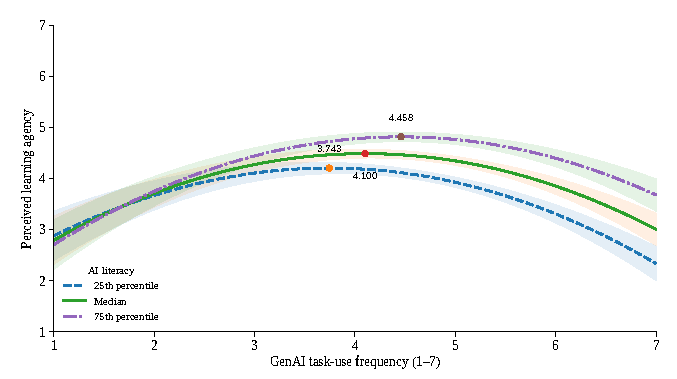
\includegraphics[width=0.8\textwidth]{fig_u_students.pdf}
\caption{Students: literacy-conditioned use--perceived learning agency association. Curves represent the 25th percentile, median, and 75th percentile of AI literacy; shaded bands denote pointwise 95\% HC3 confidence intervals for the covariate-averaged conditional mean. These are fitted curve displays, not raw observation plots. Pooled and literacy-stratified use summaries appear in Table~\ref{tab:usedist}.}
\label{fig:u_students}
\end{figure}
\vspace{-12pt}

\begin{figure}[H]

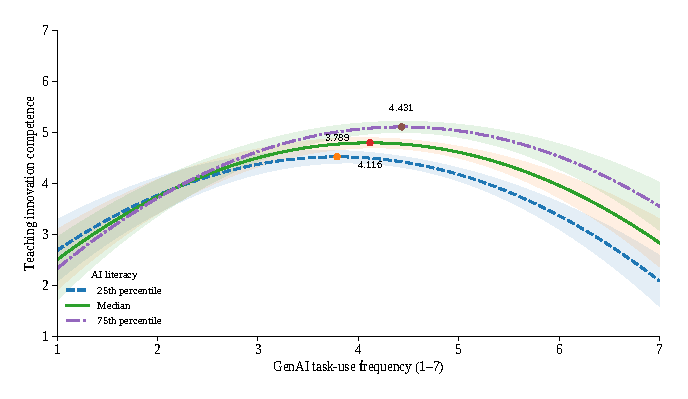
\includegraphics[width=0.8\textwidth]{fig_u_teachers.pdf}
\caption{\textls[-15]{Teachers: literacy-conditioned use--self-reported teaching innovation association. Curves represent the 25th percentile, median, and 75th percentile of AI literacy; shaded bands denote pointwise 95\% HC3 confidence intervals for the covariate-averaged conditional mean. These are fitted curve displays, not raw observation plots. Pooled and literacy-stratified use summaries appear in Table~\ref{tab:usedist}.}}
\label{fig:u_teachers}
\end{figure}

\subsection{Dimension-Level Literacy Moderation}\label{sec:dimensions}

The one-factor literacy comparison limits a unidimensional interpretation of H2. The primary interaction therefore concerns the observed, equally weighted literacy composite, not a single latent trait measured without error. Separate exploratory models yielded positive dimension-by-use interactions for awareness, practical use, critical evaluation, and ethical judgement in both cohorts (Table~\ref{tab:dimensions}). Critical evaluation had the largest interaction point estimate in each cohort. These models were fitted separately, and differences between their coefficients were not formally tested; the estimates do not establish that one dimension is statistically superior or uniquely responsible for the global interaction.

\begin{table}[H]
\caption{Dimension-specific literacy moderation of perceived capability.}
\label{tab:dimensions}
\footnotesize
\begin{adjustwidth}{-\extralength}{0cm}
\begin{tabularx}{\fulllength}{lCCCCCC}
\toprule
\textbf{Dimension} & \boldmath{$\beta_S$} & \textbf{95\% CI\boldmath{$_S$}} & \boldmath{$p_S$} & \boldmath{$\beta_T$} & \textbf{95\% CI\boldmath{$_T$}} & \boldmath{$p_T$}\\
\midrule
Awareness &\hl{0}.071 & [\hl{0}.014, \hl{0}.128] &\hl{0}.015 &\hl{0}.083 & [\hl{0}.012, \hl{0}.154] &\hl{0}.022\\
Practical use &\hl{0}.126 & [\hl{0}.067, \hl{0}.185] & <\hl{0}.001 &\hl{0}.154 & [\hl{0}.080, \hl{0}.228] & <\hl{0}.001\\
Critical evaluation &\hl{0}.168 & [\hl{0}.113, \hl{0}.223] & <\hl{0}.001 &\hl{0}.196 & [\hl{0}.125, \hl{0}.267] & <\hl{0}.001\\
Ethical judgement &\hl{0}.088 & [\hl{0}.027, \hl{0}.149] &\hl{0}.005 &\hl{0}.112 & [\hl{0}.034, \hl{0}.190] &\hl{0}.005\\
\bottomrule
\end{tabularx}
\end{adjustwidth}
\TableNote{Notes: Each row comes from a separate model substituting one literacy dimension for the global score while retaining the original use, squared use, interaction, and control structure. Coefficients are standardised dimension-by-linear-use interactions. Each model includes the corresponding dimension main effect and excludes a dimension-by-squared-use term. Coefficients from different rows are not formal tests of differences between dimensions.}
\end{table}

\vspace{-4pt}


Figures~\ref{fig:dim_students} and \ref{fig:dim_teachers} visualise the estimates and confidence intervals.

\begin{figure}[H]

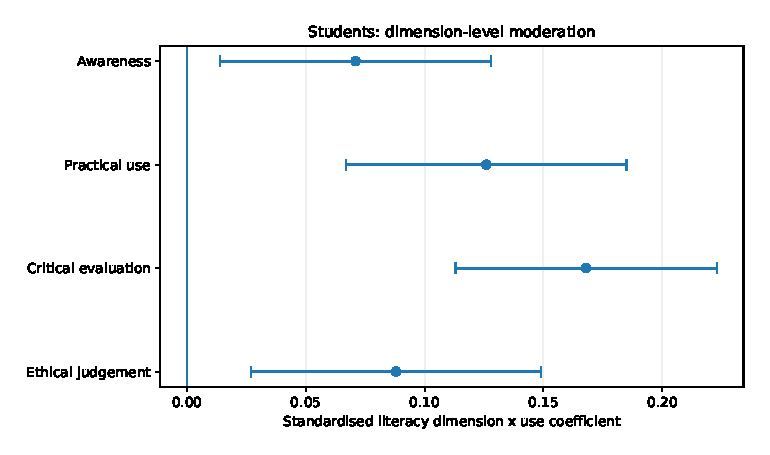
\includegraphics[width=0.8\textwidth]{fig_literacy_dimensions_students.pdf}
\caption{Students: dimension-specific literacy-by-use coefficients for perceived learning agency.}
\label{fig:dim_students}
\end{figure}
\vspace{-12pt}

\begin{figure}[H]

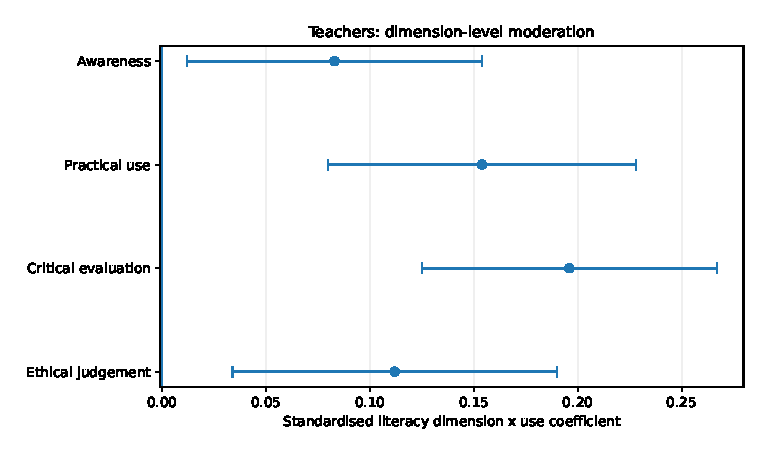
\includegraphics[width=0.8\textwidth]{fig_literacy_dimensions_teachers.pdf}
\caption{Teachers: dimension-specific literacy-by-use coefficients for self-reported teaching innovation competence.}
\label{fig:dim_teachers}
\end{figure}

Table~\ref{tab:usedecomp} separates the support-oriented and substitution-proximal use specifications. Each set of coefficients describes one substituted use index with the same literacy and control structure. The substitution-proximal squared use estimates were more strongly negative ($\beta_S=-0.249$, $\beta_T=-0.301$) than the support-oriented estimates ($\beta_S=-0.057$, $\beta_T=-0.071$), while all four literacy interactions were positive. This is a descriptive difference across separate specifications, not a formal between-index contrast; the separate models do not isolate mutually adjusted task type effects. Because the original items measure frequency rather than the actual delegation depth, the decomposition remains a sensitivity analysis of the frequency measure.

\begin{table}[H]
\caption{Exploratory decomposition of the five-item use frequency index in the capability models.}
\label{tab:usedecomp}
\small


\setlength{\tabcolsep}{3.25mm}\begin{tabular}{lcc}
\toprule
\textbf{Term} & \textbf{Students: \boldmath{$\beta$} [95\% CI]} & \textbf{Teachers: \boldmath{$\beta$} [95\% CI]}\\
\midrule
Support-oriented use, linear & \hl{0}.039 [$-$\hl{0}.020, \hl{0}.098] & \hl{0}.048 [$-$\hl{0}.025, \hl{0}.121]\\
Support-oriented use, squared & $-$\hl{0}.057 [$-$\hl{0}.097, $-$\hl{0}.017] & $-$\hl{0}.071 [$-$\hl{0}.123, $-$\hl{0}.019]\\
Literacy $\times$ support-oriented use & \hl{0}.083 [\hl{0}.031, \hl{0}.135] & \hl{0}.108 [\hl{0}.039, \hl{0}.177]\\
Substitution-proximal use, linear & $-$\hl{0}.187 [$-$\hl{0}.258, $-$\hl{0}.116] & $-$\hl{0}.164 [$-$\hl{0}.256, $-$\hl{0}.072]\\
Substitution-proximal use, squared & $-$\hl{0}.249 [$-$\hl{0}.310, $-$\hl{0}.188] & $-$\hl{0}.301 [$-$\hl{0}.384, $-$\hl{0}.218]\\
Literacy $\times$ substitution-proximal use & \hl{0}.173 [\hl{0}.117, \hl{0}.229] & \hl{0}.212 [\hl{0}.137, \hl{0}.287]\\
\bottomrule
\end{tabular}\par
\TableNote{Notes: Support-oriented = explanation, ideation, and revision items; substitution-proximal = substantial draft and complex task completion items. The two indices are fitted in separate models, each with its own linear and squared use terms and literacy interaction; coefficients are not mutually adjusted contrasts between task types. The labels are a post hoc classification of item content; the items measure task frequency, not the proportion of work delegated, verification behaviour, or task consequence.}
\end{table}

\subsection{Reliability, Trust, Control, and Institutional Sensitivity}\label{sec:sensitivity}

The reliable-core specifications preserved the central coefficients. Relative to the expanded models, the final $R^2$ values were \hl{0}.659, \hl{0}.788, \hl{0}.638, and \hl{0}.665 for student agency, student dependence, teacher innovation, and teacher dependence, respectively. Changes in the focal standardised coefficients did not exceed \hl{0}.013 (Table~\ref{tab:stability}). The literacy-only CFA factor score specifications preserved the signs and statistical significance of the focal capability and dependence coefficients. The indicator-pruning sensitivity used an explicit loading threshold of \hl{0}.60 applied to focal indicators, excluding the ancillary controls: no student indicator met the removal rule, while teacher HB1 ($\lambda=0.557$) and RK1 ($\lambda=0.551$) were removed. The student estimates were therefore unchanged in this row, and the teacher median literacy maximum changed by only 0.008 scale units. The primary scales and claims use all administered indicators.

\begin{table}[H]
\caption{Expanded versus reliable-core model stability.}
\label{tab:stability}
\small

\begin{tabularx}{\textwidth}{YCCCC}
\toprule
\textbf{Statistic} & \textbf{Student Agency} & \textbf{Student Dependence} & \textbf{Teacher Innovation} & \textbf{Teacher Dependence}\\
\midrule
Expanded $R^2$ &\hl{0}.665 &\hl{0}.793 &\hl{0}.646 &\hl{0}.671\\
Reliable-core $R^2$ &\hl{0}.659 &\hl{0}.788 &\hl{0}.638 &\hl{0}.665\\
Maximum absolute focal coefficient change &\hl{0}.009 &\hl{0}.006 &\hl{0}.013 &\hl{0}.007\\
\bottomrule
\end{tabularx}
\TableNote{Note: The reliable-core specification drops the six ancillary scales in Table~\ref{tab:controls}; the complete coefficient comparison appears in Appendix~\ref{app:coeffs}.}
\end{table}

The trust sensitivity analyses separated the substantive reliance pattern from item overlap. Using the belief-centred two-item trust score reduced the student trust coefficient from \hl{0}.329 to \hl{0}.286 (95\% CI [\hl{0}.231, \hl{0}.341], $p<0.001$) and the teacher coefficient from \hl{0}.308 to \hl{0}.271 (95\% CI [\hl{0}.194, \hl{0}.348], $p<0.001$). In models omitting trust, the dependence $R^2$ declined to \hl{0}.721 for students and \hl{0}.612 for teachers, but use, habit, and literacy retained their directions and statistical significance. Trust therefore explains a meaningful share of the reliance-related variance without being the sole basis for the dependence pathway. Table~\ref{tab:trustsens} reports the latent correlation, nested constraint, and belief-centred trust evidence. The complete set of dependence-model specifications, including trust omission, is reported once in Table~\ref{tab:depsens}.

\begin{table}[H]
\caption{Covariance-based CFA tests and belief-centred sensitivity for trust and dependence.}
\label{tab:trustsens}
\small


\setlength{\tabcolsep}{3.4mm}\begin{tabular}{lcc}
\toprule
\textbf{Statistic} & \textbf{Students} & \textbf{Teachers}\\
\midrule
Latent trust--dependence correlation &\hl{0}.806 [\hl{0}.772, \hl{0}.837] &\hl{0}.741 [\hl{0}.678, \hl{0}.797] \\
Collapsed one-factor increase, $\Delta\chi^2$ (one df) & 184.63 & 63.67 \\
Constraint $r=0.85$, $\Delta\chi^2(1)$ & 6.12, $p=0.013$ & 8.71, $p=0.003$ \\
Full-scale trust coefficient in dependence model &\hl{0}.329 [\hl{0}.280, \hl{0}.378] &\hl{0}.308 [\hl{0}.235, \hl{0}.381]\\
Belief-centred trust coefficient &\hl{0}.286 [\hl{0}.231, \hl{0}.341] &\hl{0}.271 [\hl{0}.194, \hl{0}.348]\\
Belief-centred HTMT &\hl{0}.842 [\hl{0}.804, \hl{0}.876] &\hl{0}.757 [\hl{0}.702, \hl{0}.807]\\

\bottomrule
\end{tabular}\par
\TableNote{Notes: The belief-centred trust score excludes the item that explicitly refers to willingness to rely on GenAI (TR3, Appendix~\ref{app:instrument}). Brackets are 95\% confidence intervals. The collapsed one-factor comparison is reported as a descriptive fit contrast; the $r=0.85$ comparison is a regular one-constraint test.}
\end{table}

The exceptionally high student dependence $R^2=0.793$ should be read as a within-instrument explanatory fit among conceptually related self-reports, not as predictive accuracy for an independently measured behavioural criterion. The shared method and the proximity of trust and dependence may contribute to this value even though the CFA and sensitivity evidence supports their separation.

The institutional outcome ICCs ranged from \hl{0}.024 to \hl{0}.039. Institution fixed effects and leave-one-institution-out models retained the negative squared use and positive literacy interaction signs in both capability models. The small dependence interaction ranges crossed zero, consistent with their limited explanatory contribution. Table~\ref{tab:institution} complements the fixed-effect and leave-one-out estimates with null-imposed wild cluster tests. Each reported $p$ value is the exact tail proportion over the 7776 Webb weight combinations described in Section~\ref{sec:inference}. The capability curvature and interaction test values remained below \hl{0}.05; the student dependence curvature test result was \hl{0}.059 under the cluster scheme, so this term was small in magnitude and only marginally detectable under the cluster scheme. These findings remain sensitivity evidence because the five institutions provide limited cluster-level~information.

HC3 standard errors were used because the heteroskedasticity test outcomes were significant, while the functional-form diagnostics for the final specifications did not indicate omitted low-order structure. Detailed boundary frequencies, RESET tests, influence diagnostics, institutional sensitivity, and scoring/control sensitivity results appear in Appendix~\ref{app:robust}.

\subsection{Out-of-Fold Predictive Triangulation}\label{sec:predictionresults}

Table~\ref{tab:prediction} compares linear ridge, nonlinear ridge, and the three tree-based families using pooled outer-fold predictions. Adding the prespecified square and interaction increased the capability $R^2$ from \hl{0}.514 to \hl{0}.611 for students and from \hl{0}.476 to \hl{0}.561 for teachers, with gains of \hl{0}.097 and \hl{0}.085. XGBoost added a further \hl{0}.017 and \hl{0}.018 beyond nonlinear ridge. For dependence, the two ridge specifications differed by only \hl{0}.001 in each cohort. Thus, much of the capability prediction improvement over a linear baseline was captured by the specified nonlinearity, with a smaller residual gain from the tree model. XGBoost had the highest observed pooled $R^2$ for all four outcomes; this reflects a descriptive comparison of the evaluated families, not a separately validated estimate after selecting a winning family. The teacher innovation values $R^2=0.579$, RMSE = \hl{0}.681, and outcome SD = 1.05 refer to the same 446 original-scale observations. The shared-site design estimates neither performance in a new institution nor performance in a later cohort.

\begin{table}[H]
\caption{Nested five-fold out-of-fold predictive performance by model family.}
\label{tab:prediction}
\footnotesize
\begin{adjustwidth}{-\extralength}{0cm}
\begin{tabularx}{\fulllength}{lCCCCCCC}
\toprule
\textbf{Outcome} & \textbf{Linear Ridge \boldmath{$R^2$}} & \textbf{Nonlinear Ridge \boldmath{$R^2$}} & \textbf{RF \boldmath{$R^2$}} & \textbf{XGBoost \boldmath{$R^2$}} & \textbf{LightGBM \boldmath{$R^2$}} & \textbf{Best RMSE} & \textbf{Best MAE}\\
\midrule
Student-perceived learning agency &\hl{0}.514 &\hl{0}.611 &\hl{0}.603 &\hl{0}.628 &\hl{0}.619 &\hl{0}.676 &\hl{0}.538\\
Student AI dependence &\hl{0}.762 &\hl{0}.763 &\hl{0}.741 &\hl{0}.769 &\hl{0}.757 &\hl{0}.639 &\hl{0}.507\\
Teacher teaching innovation competence &\hl{0}.476 &\hl{0}.561 &\hl{0}.546 &\hl{0}.579 &\hl{0}.567 &\hl{0}.681 &\hl{0}.542\\
Teacher AI dependence &\hl{0}.621 &\hl{0}.622 &\hl{0}.594 &\hl{0}.627 &\hl{0}.615 &\hl{0}.726 &\hl{0}.581\\
\bottomrule
\end{tabularx}
\end{adjustwidth}
\TableNote{Notes: RF = random forest. Best RMSE and MAE refer to the family with the highest pooled out-of-fold $R^2$. Differences between families are descriptive; no paired uncertainty interval for their difference is estimated here. All preprocessing and tuning were nested within the training portion of each outer fold. Hyperparameters and outer-fold performance ranges are reported in Appendix~\ref{app:ml}. Values are pooled from nested outer-fold predictions.}
\end{table}

The held-out SHAP summaries in Appendix~\ref{app:shap} describe the cross-fitted XGBoost predictions. Among the four displayed predictors, literacy made the largest mean absolute contribution to capability (\hl{0}.426 for students and \hl{0}.391 for teachers), followed by task use (\hl{0}.238 and \hl{0}.251). Trust made the largest displayed contribution to dependence (\hl{0}.343 and \hl{0}.279). These importance summaries align with the two outcome patterns but do not identify the direction of an effect, unique variance, or a causal mechanism. Their interpretation is kept separate from that of the coefficient tests and formal shape assessment.
\subsection{Hypothesis and Research Question Assessment}\label{sec:hypotheses}

H1 was supported: both cohorts met the lower slope, upper slope, and interior maximum conditions of a formal inverted U test. H2 was supported: literacy was positively associated with perceived capability and shifted the maximum rightward; separate exploratory dimension models yielded positive interactions for all four dimensions, with the largest point estimate for critical evaluation. H3 was partially supported: use, trust, and habit were positive dependence correlates and literacy was negative in both cohorts, while perceived risk was negative only among students. The teacher habit and risk estimates remain provisional because of modest reliability. The exploratory assessment was consistent with H4: both dependence increments were below \hl{0}.01, their 90\% interval upper limits were \hl{0}.0058 and \hl{0}.0031, and neither dependence model had a fitted interior maximum within 1--7 at the mean literacy. This is an interval-based statement about small nonlinear increments, not proof of exact additivity.

RQ4 indicated cross-role structural convergence rather than coefficient identity. In the pooled, fully cohort-interacted specification, the teacher-minus-student differences in squared use and literacy-by-use were $-$\hl{0}.067 (95\% CI [$-$\hl{0}.162, \hl{0}.028], $p=0.165$) and \hl{0}.046 (95\% CI [$-$\hl{0}.037, \hl{0}.129], $p=0.276$) for capability, respectively. The corresponding dependence differences were \hl{0}.055 (95\% CI [$-$\hl{0}.019, \hl{0}.129], $p=0.145$) and $-$\hl{0}.008 (95\% CI [$-$\hl{0}.079, \hl{0}.063], $p=0.826$). These intervals include zero and do not establish statistical equivalence. They indicate no detected cross-role difference in these terms, while the separate capability models both retain negative curvature and positive literacy moderation.

\section{Discussion}\label{sec:discussion}

\subsection{A Dual-Path Account of GenAI Use}\label{sec:dualpath}

The findings support two empirically different associations with the GenAI task use frequency. Perceived capability followed a literacy-conditioned inverted U: formal tests showed positive lower-range and negative upper-range slopes, and the model-implied maximum moved rightward as literacy increased. AI dependence was predominantly additive: use, habit, and trust were positively associated with reliance, literacy was negatively associated with reliance, and the nonlinear increments had 90\% interval upper limits below the exploratory 0.01 benchmark. The student dependence curve nevertheless decelerated; ``predominantly additive'' describes the small contribution of curvature rather than a literal zero coefficient.

This distinction reconciles evidence that may otherwise appear inconsistent. Intervention studies can detect benefits when assistance operates as scaffolding; withdrawal studies can reveal costs when assistance substitutes independent processing; and cross-sectional studies can report weak linear correlations when observations occupy both sides of a concave relationship~\cite{bauer2025,bastani2025,abbas2024}. The present contribution is not a universal usage quota. It is evidence that a constant-slope model discards substantial structure in perceived capability while adequately approximating dependence.

The predictive comparison also separates specified nonlinearity from generic model flexibility. The nonlinear ridge baseline recovered most of the capability prediction gain over linear ridge, whereas the incremental gain from XGBoost was smaller. This pattern is consistent with the inferential emphasis on the square and literacy interaction; it does not validate the proposed scaffolding--substitution mechanism.

The measurement analysis narrows the interpretation of the literacy result. A one-factor representation of all 12 items was inadequate, while four correlated dimensions and a second-order representation fit better. The primary moderator nevertheless remains the observed item mean. Its positive interaction describes how the use association varies with a broad literacy composite; it is not a latent-variable interaction estimate. The positive dimension-specific interactions provide complementary exploratory evidence. Critical evaluation yielded the largest point estimate, consistent with the theoretical relevance of evaluating output quality, but these separate models do not establish comparative superiority among dimensions.

The alternative trust specifications provide complementary evidence of the dependence association. Trust and dependence were distinguishable in CFA, but their high HTMT and related wording indicate that both capture neighbouring aspects of reliance. The belief-centred trust model and the model omitting trust showed that the broader dependence pattern was not confined to including the full trust score: use, habit, and literacy remained substantively important. As in the Results, the habit and perceived risk coefficients are read with the reliability caveat attached: both teacher scales fall below the 0.70 convention, so their contributions to this pathway are provisional rather than settled. Nevertheless, temporal language such as \emph{antecedent} is not warranted by a single-wave survey. Trust is best understood here as a strong, partly overlapping reliance appraisal.

The role-specific analyses showed the same architecture among students and teachers. This is not a replication on a common outcome scale. It is cross-role structural convergence: concavity and literacy moderation appeared for both perceived capability outcomes, whereas dependence \rev{was predominantly} additive. Because teachers embed GenAI use in assessment, feedback, and course design, this finding extends the governance problem beyond individual student behaviour.

\subsection{Sustainability as an Institutional Micro-Foundation}\label{sec:sustainability}

The sustainability contribution lies in the temporal problem that the two pathways imply. Responsible use asks whether a particular act of delegation is acceptable. Sustainable integration additionally asks whether repeated assistance helps institutions to renew the human judgement on which future teaching and learning depend and whether reliance remains reversible. The present survey did not measure an institutional capability stock, SDG outcomes, or long-run lock-in directly. It identifies individual-level patterns that could accumulate into these outcomes under four explicit assumptions: repeated use patterns persist; self-appraised capability tracks at least part of role performance; institutions aggregate individual routines through curriculum and assessment; and corrective opportunities are unevenly distributed.

Under these assumptions, capability calibration and dependence governance are not redundant. A user can report stronger capability while also becoming more reliant, and literacy can shift the capability maximum without eliminating habit. Sustainable higher education therefore requires an indicator system that tracks perceived and behavioural capability, verification, and reliance alongside the adoption volume. Longitudinal within-person data, post-withdrawal performance tasks, and institution-level panels are required to test the stock-and-flow proposition directly.

\subsection{Evidence-Informed Design Implications}\label{sec:implications}

The two tracks below are design implications of a cross-sectional association pattern, not interventions tested in this study. Reverse selection, unmeasured confounding, differences in task type, prior achievement, institutional support, and changes in self-appraisal remain compatible with the results. The proposals should therefore be evaluated experimentally or longitudinally before policy adoption.

The first track is \emph{\hl{capability calibration}%MDPI: Please confirm if the italics are necessary; if not, please remove them. The following highlights are the same.
}. One proposal for evaluation is that AI literacy curricula move beyond operational familiarity to critical evaluation, uncertainty recognition, task boundaries, and the deliberate decision not to delegate. Learning and professional development tasks can require independent generation before AI critique, the explicit comparison of alternatives, and the justification of accepted or rejected suggestions. The dimension-level pattern makes verification and evaluative judgement candidates for evaluation, alongside the other literacy dimensions.

The second track is \emph{\hl{dependence governance}}. The distinct dependence pattern motivates the testing of trust- and habit-focused approaches alongside literacy training. Institutions can test trust calibration measures that make uncertainty visible, require source verification, and distinguish low- from high-consequence tasks. They can also evaluate planned AI-off phases, rotating tool-free exercises, and delegation logs that make habitual patterns visible. Assessment designs that reward process, provenance, and critique connect the two tracks~\cite{joseph2025}.

Restrictions carry distributional risks. Students with disabilities, second-language learners, and those with limited access to human tutoring may rely on AI for functions not equally available elsewhere. Removing assistance without equivalent support could widen rather than narrow capability gaps. Any AI-off provision should therefore be paired with accessible alternatives, reasonable accommodations, and the monitoring of unequal burdens. This equity requirement connects the two-track architecture to SDG~4 targets concerning inclusion, relevant skills, and teacher development, while avoiding a claim that the present study demonstrates SDG effects.

\subsection{Limitations and Future Research}\label{sec:limits}

The design is cross-sectional and does not identify within-person development. The fitted curve is estimated from differences between respondents. It cannot show that a given individual first improves and then declines as use increases. Intensive use may change perceived capability, lower-capability respondents may select into intensive use, high-use respondents may appraise themselves more critically, or unmeasured task and institutional factors may generate the curvature. The model-implied maximum is therefore a statistical feature of the observed association, not an individual optimum.

All focal variables were self-reported in one instrument. Perceived learning agency and self-reported teaching innovation competence do not reflect retained performance after AI withdrawal. Use frequency does not reflect the delegation depth, task consequences, or the proportion of work completed by AI. The support-oriented versus substitution-proximal decomposition is informative but post hoc. Future instruments should distinguish between generation, revision, verification, direct delegation, task consequences, and AI-free performance.

The measurement quality remains unequal across constructs. The higher-order analysis strengthens the interpretation of AI literacy, but several teacher scales have modest reliability, and the teacher innovation AVE is slightly below 0.50. Under classical additive outcome errors that are conditionally mean-zero and unrelated to the regressors, measurement noise can reduce the precision without changing the population slopes. These assumptions are not established by reliability or AVE estimates, however. Systematic self-appraisal errors, common-method covariance, and errors in predictors or interaction terms may alter the estimated associations; the diagnostics cannot rule out measurement-related curvature. Trust and dependence are distinguishable but closely related. The next instrument development wave should separate trust beliefs from dependence-like difficulty in disengaging, using cognitive interviews, discriminant validity pretests, and, where theoretically appropriate, trait--method or bifactor models.

The convenience sample was drawn from five universities in one metropolitan setting, invitation counts were not retained, and the five clusters provide limited institutional inference. The institutional sensitivity analyses do not establish generalisability. Replication should include different regions, adoption levels, disciplines, assessment regimes, and access conditions. The joint support summaries also aggregate respondents into broad literacy strata, so uncertainty about sparsely represented local combinations remains. Hyperparameter tuning was nested, but the outer folds shared institutions, and the highest-performing family was identified descriptively from these outer results; transport to a new setting and uncertainty in family comparisons remain untested.

Future research should combine four forms of evidence: longitudinal within-person trajectories, randomised literacy and task design interventions, behavioural performance after temporary AI withdrawal, and platform telemetry or task-level delegation logs. These designs can test whether literacy causally shifts the capability maximum, whether trust precedes dependence, and whether individual patterns aggregate into institutional capability renewal or lock-in.

\section{Conclusions}\label{sec:conclusions}

Sustainable GenAI integration cannot be evaluated by adoption or use frequency alone. Across student and teacher cohorts, the GenAI task use frequency showed a formally supported, literacy-conditioned inverted U association with perceived role-specific capability. Moving from the 25th to the 75th percentile of literacy shifted the model-implied maximum by approximately 0.715 scale units for students and 0.643 for teachers. The CFA comparisons support a broad composite interpretation, and separate exploratory dimension models yielded positive interactions, with the largest point estimate for critical~evaluation.

AI dependence followed a distinct pathway. Use, habit, and trust were positive correlates; literacy was negative; and the nonlinear increments of \hl{0}.0024 and \hl{0}.0004 had 90\% interval upper bounds of \hl{0}.0058 and \hl{0}.0031, below the exploratory \hl{0}.01 benchmark. The predictive comparison similarly showed large gains from adding the specified nonlinearity for capability and minimal changes for dependence. Trust remained substantively important in the belief-centred sensitivity model, while use, habit, and literacy remained robust when trust was omitted; its conceptual proximity to dependence nevertheless warrants careful~interpretation.

The findings motivate two complementary targets for future evaluation: literacy-oriented task design and the calibration of trust and habitual reliance. The present survey does not show that either approach widens an individual's productive use range or reduces dependence. Their effectiveness, interaction, and distributional consequences should be tested with longitudinal or experimental designs that include independent performance measures and accessible alternatives to AI \hl{assistance.} %MDPI: We have noted the presence of supplementary material in the system. Please confirm whether supplementary material exists; if so, please include a "Supplementary Material" section here and ensure it is cited in the main text.


\vspace{6pt}

\authorcontributions{Conceptualisation, X.Z. and C.L.; methodology, X.Z.; software, X.Z.; validation, Y.W.; formal analysis, X.Z.; investigation, X.Z. and Y.W.; resources, C.L.; data curation, Y.W.; writing---original draft preparation, X.Z.; writing---review and editing, Y.W. and C.L.; visualisation, X.Z.; supervision, C.L.; project administration, C.L. All authors have read and agreed to the published version of the manuscript.}

\funding{This research received no external funding.}

\institutionalreview{The study was conducted in accordance with the Declaration of Helsinki and approved by the Science Research Ethics Committee of Beijing Technology and Business University (protocol code 2025-(70), approved on 2025-09-01).}

\informedconsent{Informed consent was obtained from all subjects involved in the study. The online questionnaire opened with an information page stating the purpose of the study, the voluntary nature of participation, the anonymity of the responses, and the right to withdraw at any time; respondents could access the questionnaire only after actively checking the consent box. All participants were aged 18 years or older, and no personally identifying information was collected.}

\label{sec:availability}\dataavailability{Participant-level responses, including de-identified records, are not publicly released because the consent materials did not authorise unrestricted public dissemination. Any access to such records is subject to the original consent terms and applicable institutional approvals; enquiries should be directed to the corresponding author. An analysis code attachment accompanies the manuscript, with a scoring dictionary, the CFA syntax, the regression and bootstrap routines, and the nested prediction and SHAP export workflow. It includes an output manifest specifying the model records and aggregate summaries associated with each analysis. Participant-level inputs and fitted model files are handled under the original consent terms and applicable approvals. The public, open-source release of the code is planned separately.}

\acknowledgments{\hl{The} %MDPI: Please ensure that all individuals included in this section have consented to the acknowledgement.
 \textls[-25]{authors thank the participating students, teachers, and collaborating institutions.}}

\conflictsofinterest{The authors declare no conflicts of interest.}

\abbreviations{Abbreviations}{%
The following abbreviations are used in this manuscript:\\

\noindent
\begin{tabular}{@{}ll}
AI & Artificial intelligence\\
AVE & Average variance extracted\\
CFA & Confirmatory factor analysis\\
CFI & Comparative fit index\\
CR & Composite reliability\\
GenAI & Generative artificial intelligence\\
HC3 & Heteroskedasticity-consistent standard error, type 3\\
HTMT & Heterotrait--monotrait ratio\\
MAE & Mean absolute error\\
OOF & Out-of-fold\\
RMSEA & Root mean square error of approximation\\
RMSE & Root mean squared error\\
SDG & Sustainable Development Goal\\
SHAP & Shapley additive explanations\\
SRMR & Standardized root mean square residual\\
TLI & Tucker--Lewis index\\
\end{tabular}
}

\appendixtitles{yes}
\appendixstart
\appendix



\section{English Item Map, Measurement Literature, Wording Notes, and Standardised Loadings}\label{app:instrument}

The questionnaire was administered in Chinese; the English wordings below are the reconciled back-translations. This table documents the reported item content and construct coverage; it is not a facsimile of the Chinese survey form. AI literacy dimension loadings and reliability indices come from the isolated correlated four-dimension model. Other focal loadings and reliability indices come from the corresponding full first-order measurement model. Ancillary loadings come from separate three-indicator models, which are only identified and therefore provide no fit test of their own. Construct-level descriptive statistics are reported in Table~\ref{tab:correlations}. The output manifest lists item descriptives, response frequencies, missingness counts, and covariance summaries.




\begin{table}[H] 

\caption{English item map, measurement literature and wording notes, and standardised loadings.}\label{tab:items}
\footnotesize
%\renewcommand{\arraystretch}{0.94}
%\setlength{\tabcolsep}{3pt}


%\centering %% If there is a figure in wide page, please release command \centering

\begin{adjustwidth}{-\extralength}{0cm}
%\centering %% If there is a figure in wide page, please release command \centering
\setlength{\tabcolsep}{2.5mm}\begin{tabular}{p{1.2cm}p{4cm}p{5cm}p{4cm}cc}
\toprule
\textbf{Code} & \textbf{Construct} & \textbf{Item Wording} & \textbf{Measurement Literature/Wording Notes} & \boldmath{$\lambda_S$} & \boldmath{$\lambda_T$}\\
\midrule



\hl{AIL-AW1} %MDPI: We have added lines to make it easier to read. Please confirm the changes.
 & AI literacy--awareness & I can recognise common functions for which GenAI systems are used. & Wang et al.~\cite{wang2023}; parallel role-neutral wording &\hl{0}.704 &\hl{0}.662 \\\midrule
AIL-AW2 & AI literacy--awareness & I understand that GenAI output is generated probabilistically and can be inaccurate. & Wang et al.~\cite{wang2023}; GenAI-specific adaptation &\hl{0}.742 &\hl{0}.701 \\\midrule
AIL-AW3 & AI literacy--awareness & I can identify situations in which GenAI is and is not an appropriate tool. & Wang et al.~\cite{wang2023}; GenAI-specific adaptation &\hl{0}.706 &\hl{0}.673 \\\midrule
AIL-PU1 & AI literacy--practical use & I can formulate prompts that communicate the task and constraints clearly. & Wang et al.~\cite{wang2023}; GenAI-specific adaptation &\hl{0}.751 &\hl{0}.711 \\\midrule
AIL-PU2 & AI literacy--practical use & I can refine my instructions when an initial GenAI response is inadequate. & Wang et al.~\cite{wang2023}; GenAI-specific adaptation &\hl{0}.798 &\hl{0}.754 \\\midrule
AIL-PU3 & AI literacy--practical use & I can integrate useful GenAI output into my own learning/teaching work. & Role-specific task referent &\hl{0}.752 &\hl{0}.709 \\\midrule
AIL-CE1 & AI literacy--critical evaluation & I can assess whether a GenAI response is factually and logically sound. & Wang et al.~\cite{wang2023}; GenAI-specific adaptation &\hl{0}.821 &\hl{0}.774 \\\midrule
AIL-CE2 & AI literacy--critical evaluation & I verify important GenAI claims using independent evidence. & Wang et al.~\cite{wang2023}; GenAI-specific adaptation &\hl{0}.792 &\hl{0}.801 \\\midrule
AIL-CE3 & AI literacy--critical evaluation & I can detect omissions, bias, or unjustified confidence in GenAI output. & Wang et al.~\cite{wang2023}; GenAI-specific adaptation &\hl{0}.837 &\hl{0}.817 \\\midrule
AIL-EJ1 & AI literacy--ethical judgement & I consider privacy and data-protection risks before using GenAI. & Wang et al.~\cite{wang2023}; GenAI-specific adaptation &\hl{0}.683 &\hl{0}.642 \\\midrule
AIL-EJ2 & AI literacy--ethical judgement & I consider authorship, attribution, and academic/professional integrity. & Role-specific contextual adaptation &\hl{0}.724 &\hl{0}.691 \\\midrule
AIL-EJ3 & AI literacy--ethical judgement & I retain personal responsibility for decisions informed by GenAI. & GenAI governance adaptation &\hl{0}.728 &\hl{0}.702 \\\midrule
USE1 & GenAI task use frequency & Frequency of using GenAI to obtain explanations or clarify concepts. & Student: learning; teacher: instructional concepts &\hl{0}.702 &\hl{0}.681 \\\midrule






USE2 & GenAI task use frequency & Frequency of using GenAI to generate ideas or initial plans. & Parallel role-specific referent &\hl{0}.738 &\hl{0}.704 \\\midrule
USE3 & GenAI task use frequency & Frequency of using GenAI to review, revise, or improve existing work. & Parallel role-specific referent &\hl{0}.756 &\hl{0}.742 \\\midrule
USE4 & GenAI task use frequency & Frequency of using GenAI to produce substantial drafts or task outputs. & Substitution-proximal classification &\hl{0}.729 &\hl{0}.713 \\\midrule
USE5 & GenAI task use frequency & Frequency of using GenAI to complete complex tasks that would otherwise require substantial independent work. & Substitution-proximal classification &\hl{0}.671 &\hl{0}.645 \\\midrule
TR1 & Trust in GenAI & I expect GenAI to provide generally competent assistance for suitable tasks. & Trust-in-automation adaptation~\cite{lee2004,hoff2015} &\hl{0}.664 &\hl{0}.611 \\

\bottomrule
\end{tabular}
\end{adjustwidth}
\end{table}

\begin{table}[H]\ContinuedFloat

\caption{{\em Cont.}}
\label{tab:items}
\footnotesize
%\renewcommand{\arraystretch}{0.94}
%\setlength{\tabcolsep}{3pt}


%\centering %% If there is a figure in wide page, please release command \centering

\begin{adjustwidth}{-\extralength}{0cm}
%\centering %% If there is a figure in wide page, please release command \centering
\setlength{\tabcolsep}{2.5mm}\begin{tabular}{p{1.2cm}p{4cm}p{5cm}p{4cm}cc}
\toprule
\textbf{Code} & \textbf{Construct} & \textbf{Item Wording} & \textbf{Measurement Literature/Wording Notes} & \boldmath{$\lambda_S$} & \boldmath{$\lambda_T$}\\
\midrule




TR2 & Trust in GenAI & I believe GenAI recommendations are dependable when I can verify them. & Belief-centred item &\hl{0}.711 &\hl{0}.653 \\\midrule



TR3 & Trust in GenAI & I am willing to rely on GenAI when completing relevant tasks. & Full-scale item; excluded from belief-centred sensitivity &\hl{0}.735 &\hl{0}.716 \\\midrule
HB1 & Habitual GenAI use & Using GenAI has become something I do automatically in relevant situations. & UTAUT2/continuance adaptation~\cite{limayem2007,venkatesh2012} &\hl{0}.652 &\hl{0}.557 \\\midrule






HB2 & Habitual GenAI use & When a suitable task appears, using GenAI is one of my first reactions. & UTAUT2/continuance adaptation &\hl{0}.701 &\hl{0}.625 \\\midrule
HB3 & Habitual GenAI use & I use GenAI with little conscious deliberation in familiar task settings. & Habit automaticity adaptation &\hl{0}.721 &\hl{0}.679 \\\midrule
RK1 & Perceived GenAI risk & GenAI errors could lead me to make poor learning/teaching decisions. & GenAI-specific risk adaptation &\hl{0}.614 &\hl{0}.551 \\\midrule
RK2 & Perceived GenAI risk & Relying on GenAI may weaken my ability to evaluate work independently. & GenAI-specific risk adaptation &\hl{0}.662 &\hl{0}.603 \\\midrule
RK3 & Perceived GenAI risk & Using GenAI for consequential tasks may create academic/professional problems. & Role-specific consequence adaptation &\hl{0}.725 &\hl{0}.667 
\\\midrule





AG1 & Perceived learning agency & I set clear goals for my own learning. & Student version; agency/self-regulation adaptation~\cite{bandura2001,xia2026} &\hl{0}.692 & --- \\\midrule
AG2 & Perceived learning agency & I decide how to approach difficult learning tasks. & Student version &\hl{0}.724 & --- \\\midrule







AG3 & Perceived learning agency & I persist when learning becomes difficult. & Student version &\hl{0}.681 & --- \\\midrule
AG4 & Perceived learning agency & I monitor whether my current learning strategy is working. & Student version &\hl{0}.746 & --- \\\midrule
AG5 & Perceived learning agency & I revise my approach when my progress is inadequate. & Student version &\hl{0}.771 & --- \\\midrule
AG6 & Perceived learning agency & I can explain the reasoning behind my learning decisions. & Student version &\hl{0}.735 & --- \\\midrule
AG7 & Perceived learning agency & I take responsibility for the quality of my learning outcomes. & Student version &\hl{0}.758 & --- \\\midrule
TI1 & Teaching innovation competence & I can identify teaching problems that require a new instructional approach. & Teacher version; teaching-innovation adaptation~\cite{zhaiTeacher2025,mishra2023} & --- &\hl{0}.648 \\\midrule
TI2 & Teaching innovation competence & I can design learning activities that use digital tools purposefully. & Teacher version & --- &\hl{0}.714 \\\midrule
TI3 & Teaching innovation competence & I adapt instructional materials to different learner needs. & Teacher version & --- &\hl{0}.681 \\\midrule
TI4 & Teaching innovation competence & I evaluate whether an instructional innovation improves learning. & Teacher version & --- &\hl{0}.731 \\\midrule







TI5 & Teaching innovation competence & I can revise AI-supported teaching designs after evidence or feedback. & Teacher version; GenAI adaptation & --- &\hl{0}.708 \\\midrule
TI6 & Teaching innovation competence & I can integrate GenAI without surrendering professional judgement. & Teacher version; GenAI adaptation & --- &\hl{0}.692 \\\midrule



DEP-S1 & Student AI dependence & I find it difficult to begin some learning tasks without GenAI assistance. & Dependence-on-AI adaptation~\cite{morales2024} &\hl{0}.778 & --- \\\midrule
DEP-S2 & Student AI dependence & I feel less confident completing familiar academic tasks when GenAI is unavailable. & Student version &\hl{0}.803 & --- \\\midrule
DEP-S3 & Student AI dependence & I rely on GenAI even when I could complete the task independently. & Student version &\hl{0}.827 & --- \\\midrule
DEP-S4 & Student AI dependence & I repeatedly check GenAI before finalising my own answer. & Student version &\hl{0}.756 & --- \\


\bottomrule
\end{tabular}
\end{adjustwidth}
\end{table}

\begin{table}[H]\ContinuedFloat

\caption{{\em Cont.}}
\label{tab:items}
\footnotesize
%\renewcommand{\arraystretch}{0.94}
%\setlength{\tabcolsep}{3pt}


%\centering %% If there is a figure in wide page, please release command \centering

\begin{adjustwidth}{-\extralength}{0cm}
%\centering %% If there is a figure in wide page, please release command \centering
\setlength{\tabcolsep}{2.5mm}\begin{tabular}{p{1.2cm}p{4cm}p{5cm}p{4cm}cc}
\toprule
\textbf{Code} & \textbf{Construct} & \textbf{Item Wording} & \textbf{Measurement Literature/Wording Notes} & \boldmath{$\lambda_S$} & \boldmath{$\lambda_T$}\\
\midrule




DEP-S5 & Student AI dependence & Interrupting access to GenAI would disrupt my usual learning process. & Student version &\hl{0}.812 & --- \\\midrule




DEP-S6 & Student AI dependence & I prefer GenAI guidance to making an unaided judgement. & Student version &\hl{0}.785 & --- \\\midrule





DEP-S7 & Student AI dependence & I use GenAI longer or more often than I originally intend. & Student version &\hl{0}.831 & --- \\\midrule







DEP-S8 & Student AI dependence & I would find it uncomfortable to complete important learning tasks without GenAI. & Student version &\hl{0}.818 & --- \\\midrule
DEP-T1 & Teacher AI dependence & I find it difficult to begin some teaching tasks without GenAI assistance. & Teacher-context reliance item; related construct literature discussed in Section~\ref{sec:measures} & --- &\hl{0}.703 \\\midrule
DEP-T2 & Teacher AI dependence & My usual preparation process would be disrupted if GenAI were unavailable. & Teacher role adaptation & --- &\hl{0}.758 \\\midrule
DEP-T3 & Teacher AI dependence & I rely on GenAI even for tasks I could complete independently. & Teacher role adaptation & --- &\hl{0}.781 \\\midrule
DEP-T4 & Teacher AI dependence & I prefer GenAI suggestions to making an unaided instructional judgement. & Teacher role adaptation & --- &\hl{0}.712 \\\midrule
DEP-T5 & Teacher AI dependence & I would find it uncomfortable to complete important teaching tasks without GenAI. & Teacher role adaptation & --- &\hl{0}.736 \\







PE1 & Performance expectancy & Using GenAI improves the quality of my learning/teaching work. & Venkatesh et al.~\cite{venkatesh2012}; role-specific GenAI adaptation &\hl{0}.642 &\hl{0}.623 \\\midrule
PE2 & Performance expectancy & Using GenAI enables me to complete relevant tasks more efficiently. & Venkatesh et al.~\cite{venkatesh2012}; role-specific GenAI adaptation &\hl{0}.671 &\hl{0}.652 \\\midrule
PE3 & Performance expectancy & GenAI is useful for accomplishing important learning/teaching tasks. & Venkatesh et al.~\cite{venkatesh2012}; role-specific GenAI adaptation &\hl{0}.629 &\hl{0}.607 \\\midrule





EE1 & Effort expectancy & Learning to use GenAI for my tasks is easy for me. & Venkatesh et al.~\cite{venkatesh2012}; GenAI adaptation &\hl{0}.611 &\hl{0}.579 \\\midrule
EE2 & Effort expectancy & My interaction with GenAI is clear and understandable. & Venkatesh et al.~\cite{venkatesh2012}; GenAI adaptation &\hl{0}.648 &\hl{0}.626 \\\midrule
EE3 & Effort expectancy & It is easy for me to become skilful at using GenAI. & Venkatesh et al.~\cite{venkatesh2012}; GenAI adaptation &\hl{0}.615 &\hl{0}.595 \\\midrule
SI1 & Social influence & People who are important to me think that I should use GenAI for relevant tasks. & Venkatesh et al.~\cite{venkatesh2012}; role-specific GenAI adaptation &\hl{0}.619 &\hl{0}.588 \\\midrule
SI2 & Social influence & People whose opinions I value encourage me to use GenAI. & Venkatesh et al.~\cite{venkatesh2012}; GenAI adaptation &\hl{0}.656 &\hl{0}.632 \\\midrule
SI3 & Social influence & People in my study/work environment commonly expect GenAI to be used. & Venkatesh et al.~\cite{venkatesh2012}; role-specific adaptation &\hl{0}.610 &\hl{0}.603 \\\midrule





FC1 & Facilitating conditions & I have the technical resources needed to use GenAI. & Venkatesh et al.~\cite{venkatesh2012}; GenAI adaptation &\hl{0}.648 &\hl{0}.628 \\\midrule
FC2 & Facilitating conditions & I have the knowledge and support needed to use GenAI effectively. & Venkatesh et al.~\cite{venkatesh2012}; GenAI adaptation &\hl{0}.673 &\hl{0}.657 \\\midrule
FC3 & Facilitating conditions & GenAI is compatible with the digital systems available for my learning/teaching work. & Venkatesh et al.~\cite{venkatesh2012}; role-specific adaptation &\hl{0}.636 &\hl{0}.620 \\\midrule




EQ1 & Educational equity & GenAI gives people with fewer educational resources better access to support. & Study-specific SDG~4-oriented ancillary item &\hl{0}.586 &\hl{0}.575 \\\midrule
EQ2 & Educational equity & GenAI can reduce differences in access to explanations or professional assistance. & Study-specific SDG~4-oriented ancillary item &\hl{0}.643 &\hl{0}.616 \\



\bottomrule
\end{tabular}
\end{adjustwidth}
\end{table}

\begin{table}[H]\ContinuedFloat

\caption{{\em Cont.}}
\label{tab:items}
\footnotesize
%\renewcommand{\arraystretch}{0.94}
%\setlength{\tabcolsep}{3pt}


%\centering %% If there is a figure in wide page, please release command \centering

\begin{adjustwidth}{-\extralength}{0cm}
%\centering %% If there is a figure in wide page, please release command \centering
\setlength{\tabcolsep}{2.5mm}\begin{tabular}{p{1.2cm}p{4cm}p{5cm}p{4cm}cc}
\toprule
\textbf{Code} & \textbf{Construct} & \textbf{Item Wording} & \textbf{Measurement Literature/Wording Notes} & \boldmath{$\lambda_S$} & \boldmath{$\lambda_T$}\\
\midrule



EQ3 & Educational equity & The benefits of GenAI are accessible across learners/teachers with different backgrounds. & Study-specific SDG~4-oriented ancillary item &\hl{0}.609 &\hl{0}.592 \\\midrule





LLL1 & Lifelong learning orientation & GenAI encourages me to continue learning beyond immediate task requirements. & Study-specific lifelong learning ancillary item &\hl{0}.614 &\hl{0}.596 \\\midrule
LLL2 & Lifelong learning orientation & I use GenAI to explore knowledge or skills beyond what is currently required. & Study-specific lifelong learning ancillary item &\hl{0}.660 &\hl{0}.639 \\\midrule
LLL3 & Lifelong learning orientation & Using GenAI increases my willingness to update my knowledge and methods. & Study-specific lifelong learning ancillary item &\hl{0}.632 &\hl{0}.608 \\
\bottomrule
\end{tabular}
\end{adjustwidth}




%\centering %% If there is a figure in wide page, please release command \centering
\TableNote{Notes for Table~\ref{tab:items}: References identify the measurement or conceptual literature associated with a construct; a first-row reference applies to the subsequent rows of that construct unless noted otherwise. Wording notes distinguish between GenAI-specific and role-specific adaptation. Entries without a citation document the study wording without attribution to a particular validated instrument. The English text is a reconciled back-translation.}

\end{table}


Scoring: literacy, trust, habit, risk, capability, dependence, and the six ancillary scales use seven-point agreement responses; use frequency uses 1 = never to 7 = multiple times per day. Except where explicitly identified as CFA factor score sensitivity models, analyses use unweighted item means. No item is reverse-scored.

The item summary record covers 41 focal student items and 37 focal teacher items, with 659 and 446 valid responses per item and no missing core responses. Item means range from 4.053 to 4.772 among students and 3.991 to 4.823 among teachers; the corresponding item standard deviation ranges are 1.282--1.662 and 1.239--1.542. Across items, the proportions selecting category 1 range within 0.61--5.31\% and 0.22--6.05\%, while the proportions selecting category 7 range within 3.95--14.87\% and 3.59--10.99\%, respectively. The item-level export retains all seven category counts in questionnaire order.

\begin{table}[H]
\caption{Background, access, and screening items included in the role-specific questionnaire.}\label{tab:background}
\footnotesize
\begin{adjustwidth}{-\extralength}{0cm}
\begin{tabularx}{\fulllength}{p{1.45cm}p{5.6cm}Yp{3.1cm}}
\toprule
\textbf{Code} & \textbf{Question Stem} & \textbf{Response Format} & \textbf{Source/Use}\\
\midrule
\hl{BG1} %MDPI: We have added lines to make it easier to read. Please confirm.
 & Which version of the questionnaire applies to you? & Student/teacher; routing item & Study-developed background item\\\midrule
BG2 & What is your gender? & Woman/man/another identity/prefer not to say & Study-developed demographic item\\\midrule
BG3 & What is your age? & Age in completed years & Study-developed demographic item\\\midrule
BG4 & What is your principal disciplinary field? & Humanities/social sciences; business/economics; STEM; education; health; arts; other & Study-developed background item\\\midrule
BG5-S/BG5-T & What is your current year of study?/How many years have you worked in higher education? & Study year 1--5 (5 = fifth year or above)/completed years & Role-specific background item\\\midrule
BG6 & At which participating institution are you enrolled or employed? & Five anonymised institution codes & Sampling and clustering variable\\\midrule
BG7-S/BG7-T & What qualification are you currently pursuing?/What is your highest completed qualification and academic rank? & Qualification recorded descriptively; teacher rank 1 = assistant, 2 = lecturer, 3 = associate professor, 4 = professor & Role-specific professional background item\\\midrule




BG8 & How long have you used generative AI tools? & 0 = never; 1 = $<3$ months; 2 = 3--6; 3 = 7--12; 4 = 13--24; 5 = $>24$ months & AI tenure control\\

\bottomrule
\end{tabularx}
\end{adjustwidth}
\end{table}

\begin{table}[H]\ContinuedFloat

\caption{{\em Cont.}}
\label{tab:background}
\footnotesize
\begin{adjustwidth}{-\extralength}{0cm}
\begin{tabularx}{\fulllength}{p{1.45cm}p{5.6cm}Yp{3.1cm}}
\toprule
\textbf{Code} & \textbf{Question Stem} & \textbf{Response Format} & \textbf{Source/Use}\\
\midrule



BG9 & Overall, how often do you use generative AI? & Same seven frequency categories as Section~\ref{sec:measures} & Overall-frequency control\\\midrule






QC1 & To confirm attention, please select ``Agree'' for this statement. & Seven-point agreement scale & Directed-response attention check\\\midrule
QC2 & To confirm attention, please select ``Strongly disagree'' for this statement. & Seven-point agreement scale & Directed-response attention check\\\midrule
META-T & Questionnaire completion time & Automatically recorded in seconds & Screening metadata; threshold in Section~\ref{sec:design}\\
\bottomrule
\end{tabularx}
\end{adjustwidth}
\end{table}


\section{{Complete Coefficients in the Expanded and Reliable-Core Specifications}}\label{app:coeffs}

\vspace{-4pt}


\setlength{\tabcolsep}{3.5pt}
\begin{table}[H] 
\caption{\hl{Complete} %MDPI: We connected lines, please confirm.
 standardised coefficients in expanded (E) and reliable-core (C) specifications.}\label{tab:fullcoeffs}
 \footnotesize

\begin{adjustwidth}{-\extralength}{0cm}
%\centering %% If there is a figure in wide page, please release command \centering
\setlength{\tabcolsep}{1.37mm}\begin{tabular}{p{4cm}*{8}{p{1.5cm}}}

\toprule
& \multicolumn{2}{c}{\textbf{Student Agency}} & \multicolumn{2}{c}{\textbf{Student Dependence}} & \multicolumn{2}{c}{\textbf{Teacher Innovation}} & \multicolumn{2}{c}{\textbf{Teacher Dependence}}\\
\cmidrule(l){2-9}
\multirow{-2.5}{*}{\textbf{\hl{Variable} %MDPI: We merged these two rows for this cell, please confirm, the following highlights are the same.
}} & \textbf{E} & \textbf{C} & \textbf{E} & \textbf{C} & \textbf{E} & \textbf{C} & \textbf{E} & \textbf{C}\\
\midrule



AI literacy &\hl{0}.487~*** &\hl{0}.480~*** & $-0.222$~*** & $-0.218$~*** &\hl{0}.487~*** &\hl{0}.478~*** & $-0.279$~*** & $-0.272$~***\\
GenAI task use frequency & $-0.171$~*** & $-0.165$~*** &\hl{0}.167~*** &\hl{0}.173~*** & $-0.151$~** & $-0.144$~** &\hl{0}.299~*** &\hl{0}.305~***\\
Task use frequency squared & $-0.293$~*** & $-0.284$~*** & $-0.045$~* & $-0.042$~* & $-0.360$~*** & $-0.347$~*** &\hl{0}.010 &\hl{0}.012\\
Literacy $\times$ task use frequency &\hl{0}.200~*** &\hl{0}.195~*** &\hl{0}.002 &\hl{0}.004 &\hl{0}.246~*** &\hl{0}.237~*** & $-0.006$ & $-0.004$\\
Trust in GenAI & $-0.012$ & $-0.010$ &\hl{0}.329~*** &\hl{0}.323~*** &\hl{0}.012 &\hl{0}.014 &\hl{0}.308~*** &\hl{0}.301~***\\
Habitual GenAI use & $-0.035$ & $-0.031$ &\hl{0}.232~*** &\hl{0}.228~*** & $-0.021$ & $-0.018$ &\hl{0}.224~*** &\hl{0}.219~***\\
Perceived GenAI risk &\hl{0}.140~*** &\hl{0}.134~*** & $-0.083$~** & $-0.079$~** &\hl{0}.074 &\hl{0}.071 & $-0.051$ & $-0.047$\\
Performance expectancy &\hl{0}.061~* & --- &\hl{0}.018 & --- &\hl{0}.074~* & --- &\hl{0}.012 & ---\\
Effort expectancy &\hl{0}.034 & --- & $-0.028$ & --- &\hl{0}.041 & --- & $-0.021$ & ---\\
Social influence &\hl{0}.012 & --- &\hl{0}.055~* & --- &\hl{0}.019 & --- &\hl{0}.063~* & ---\\
Facilitating conditions &\hl{0}.049 & --- & $-0.006$ & --- &\hl{0}.058 & --- &\hl{0}.017 & ---\\
Educational equity &\hl{0}.037 & --- & $-0.031$ & --- &\hl{0}.046 & --- & $-0.024$ & ---\\
Lifelong learning orientation &\hl{0}.068~* & --- & $-0.022$ & --- &\hl{0}.081~* & --- & $-0.018$ & ---\\




Gender (woman = 1) &\hl{0}.029 &\hl{0}.031 & $-0.024$ & $-0.023$ &\hl{0}.018 &\hl{0}.020 & $-0.033$ & $-0.032$\\
Gender: another identity &\hl{0}.008 &\hl{0}.009 & $-$0.006 & $-$0.005 &\hl{0}.012 &\hl{0}.014 & $-$0.009 & $-$0.008\\
Gender: prefer not to say & $-$0.005 & $-$0.004 &\hl{0}.007 &\hl{0}.006 & $-$0.008 & $-$0.006 &\hl{0}.005 &\hl{0}.004\\
Age/teaching experience &\hl{0}.044 &\hl{0}.046 & $-0.051$ & $-0.049$ &\hl{0}.057 &\hl{0}.059 & $-0.043$ & $-0.041$\\


%\bottomrule
%\end{tabular}
%\end{adjustwidth}
%\end{table}
%
%\begin{table}[H]\ContinuedFloat
%%\small
%\caption{{\em Cont.}}
%
%\label{tab:fullcoeffs}
% \footnotesize
%
%\begin{adjustwidth}{-\extralength}{0cm}
%%\centering %% If there is a figure in wide page, please release command \centering
%\setlength{\tabcolsep}{1.37mm}\begin{tabular}{p{4cm}*{8}{p{1.5cm}}}
%
%\toprule
%& \multicolumn{2}{c}{\textbf{Student Agency}} & \multicolumn{2}{c}{\textbf{Student Dependence}} & \multicolumn{2}{c}{\textbf{Teacher Innovation}} & \multicolumn{2}{c}{\textbf{Teacher Dependence}}\\
%\cmidrule(l){2-9}
%\multirow{-2.5}{*}{\textbf{\hl{Variable} %MDPI: We merged these two rows for this cell, please confirm, the following highlights are the same.
%}} & \textbf{E} & \textbf{C} & \textbf{E} & \textbf{C} & \textbf{E} & \textbf{C} & \textbf{E} & \textbf{C}\\
%\midrule


Study year/academic rank &\hl{0}.031 &\hl{0}.033 &\hl{0}.018 &\hl{0}.020 &\hl{0}.045 &\hl{0}.047 &\hl{0}.022 &\hl{0}.024\\
Discipline: business/economics &\hl{0}.022 &\hl{0}.024 &\hl{0}.037 &\hl{0}.039 &\hl{0}.028 &\hl{0}.030 &\hl{0}.041 &\hl{0}.043\\
Discipline: STEM &\hl{0}.047 &\hl{0}.049 &\hl{0}.029 &\hl{0}.031 &\hl{0}.052 &\hl{0}.054 &\hl{0}.036 &\hl{0}.038\\
Discipline: education &\hl{0}.036 &\hl{0}.038 & $-0.012$ & $-0.010$ &\hl{0}.063 &\hl{0}.065 & $-0.008$ & $-0.006$\\
Discipline: health &\hl{0}.019 &\hl{0}.021 &\hl{0}.024 &\hl{0}.026 &\hl{0}.033 &\hl{0}.035 &\hl{0}.028 &\hl{0}.030\\
Discipline: arts &\hl{0}.011 &\hl{0}.013 &\hl{0}.017 &\hl{0}.019 &\hl{0}.016 &\hl{0}.018 &\hl{0}.020 &\hl{0}.022\\
Discipline: other &\hl{0}.008 &\hl{0}.010 &\hl{0}.012 &\hl{0}.014 &\hl{0}.010 &\hl{0}.012 &\hl{0}.015 &\hl{0}.017\\
AI tenure &\hl{0}.038 &\hl{0}.040 &\hl{0}.071~* &\hl{0}.073~* &\hl{0}.052 &\hl{0}.055 &\hl{0}.084~* &\hl{0}.086~*\\
Overall AI use frequency & $-0.022$ & $-0.020$ &\hl{0}.092~** &\hl{0}.095~** & $-0.018$ & $-0.015$ &\hl{0}.107~** &\hl{0}.110~**\\
\midrule
$R^2$ &\hl{0}.665 &\hl{0}.659 &\hl{0}.793 &\hl{0}.788 &\hl{0}.646 &\hl{0}.638 &\hl{0}.671 &\hl{0}.665\\
Observations & 659 & 659 & 659 & 659 & 446 & 446 & 446 & 446\\
\bottomrule
\end{tabular}
\end{adjustwidth}
\TableNote{Notes: Coefficients are standardised; the reference discipline is humanities/social sciences. E = expanded specification; C = reliable-core specification. The six ancillary scale scores are omitted from C because $\alpha<0.70$ in at least one cohort. All demographics, discipline indicators, AI tenure, and overall use frequency remain in both specifications. * $p<0.05$, ** $p<0.01$, *** $p<0.001$.}
\end{table}


\section{Distributional Support, Sensitivity Models, and Diagnostics}\label{app:robust}


\vspace{-4pt}

\begin{table}[H]
\caption{\hl{Use frequency} %MDPI: We merged the two tables into one. Please confirm the changes.
 distribution and pooled and literacy-stratified support for the conditional~maxima.}\label{tab:usedist}
\footnotesize
\begin{adjustwidth}{-\extralength}{0cm}
\begin{tabularx}{\fulllength}{llCCCCC}
\toprule
\multicolumn{3}{l}{\textbf{Pooled Cohort Summary}} & \multicolumn{2}{c}{\textbf{Students}} & \multicolumn{2}{c}{\textbf{Teachers}}\\
\midrule
\multicolumn{3}{l}{Observed range} & \multicolumn{2}{c}{1.00--7.00} & \multicolumn{2}{c}{1.00--7.00}\\
\multicolumn{3}{l}{5th/25th/50th/75th/95th percentile} & \multicolumn{2}{c}{2.60/3.80/4.60/5.40/6.60} & \multicolumn{2}{c}{2.60/3.60/4.40/5.20/6.20}\\
\multicolumn{3}{l}{RCS knot locations (5 knots) }& \multicolumn{2}{c}{2.60/3.99/4.60/5.20/6.60} & \multicolumn{2}{c}{2.60/3.60/4.40/5.00/6.20}\\
\multicolumn{3}{l}{Cases within $\pm0.5$ of low-literacy maximum} & \multicolumn{2}{c}{177 }& \multicolumn{2}{c}{143}\\
\multicolumn{3}{l}{Cases within $\pm0.5$ of median-literacy maximum} & \multicolumn{2}{c}{214 }&\multicolumn{2}{c}{ 142}\\
\multicolumn{3}{l}{Cases within $\pm0.5$ of high-literacy maximum }& \multicolumn{2}{c}{229 }& \multicolumn{2}{c}{146}\\
\multicolumn{3}{l}{Cases beyond low/median/high maximum} & \multicolumn{2}{c}{509/431/351 }& \multicolumn{2}{c}{320/268/200}\\
\multicolumn{3}{l}{Largest squared term change after influence deletion} & \multicolumn{2}{c}{4.1\% }& \multicolumn{2}{c}{4.3\%}\\
\multicolumn{3}{l}{Largest interaction term change after influence deletion} & \multicolumn{2}{c}{3.8\% }& \multicolumn{2}{c}{4.0\%}\\
\multicolumn{3}{l}{RCS basis degrees of freedom} & \multicolumn{2}{c}{4 total; 3 nonlinear} & \multicolumn{2}{c}{4 total; 3 nonlinear}\\
\midrule
%\end{tabularx}
%\vspace{4pt}
%\begin{tabularx}{\fulllength}{llCCCCC}
%\toprule
Cohort & Literacy stratum & $n$ & Use $Q_{.05}/Q_{.50}/Q_{.95}$ & $n$ near maximum & $n$ below & $n$ above\\
\midrule
Students & Lower & 186 & 2.80/4.60/6.55 & 57 & 31 & 155\\
Students & Middle & 300 & 2.60/4.60/6.60 & 93 & 100 & 200\\
Students & Upper & 173 & 2.40/4.40/6.40 & 60 & 91 & 82\\
Teachers & Lower & 115 & 2.60/4.20/6.06 & 37 & 33 & 82\\
Teachers & Middle & 219 & 2.58/4.40/6.20 & 73 & 93 & 126\\
Teachers & Upper & 112 & 2.71/4.60/6.49 & 30 & 53 & 59\\
\bottomrule
\end{tabularx}
\end{adjustwidth}
\TableNote{All quantiles use type-7 linear interpolation on the same five-item use score. Lower, middle, and upper literacy strata are $L\le Q_{.25}$, $Q_{.25}<L<Q_{.75}$, and $L\ge Q_{.75}$; ties remain together. Each stratified row uses the corresponding low-, median-, or high-literacy maximum. The local window includes both endpoints of $\pm0.5$; below/above counts exclude exact ties. Pooled counts describe marginal support, while the stratified rows describe joint~support.}
\end{table}


\vspace{-12pt}


\begin{table}[H]
\caption{Observed-bound slope sensitivity at the minimum and maximum of the 1--7 use scale.}\label{tab:boundslopes}
\small
\setlength{\tabcolsep}{3pt}
\begin{tabularx}{\textwidth}{Yccc}
\toprule
\textbf{Cohort/Literacy} & \textbf{Slope at Use = 1 [95\% CI]} & \textbf{Slope at Use = 7 [95\% CI]} & \textbf{Observed-Bound \boldmath{$U$}-Test \boldmath{$p$}}\\
\midrule
Students, 25th &\hl{0}.968 [\hl{0}.721, 1.214] & $-$1.149 [$-$1.357, $-$\hl{0}.941] & <\hl{0}.001\\
Students, median & 1.094 [\hl{0}.847, 1.340] & $-$1.023 [$-$1.225, $-$\hl{0}.821] & <\hl{0}.001\\
Students, 75th & 1.220 [\hl{0}.970, 1.471] & $-$\hl{0}.897 [$-$1.097, $-$\hl{0}.697] & <\hl{0}.001\\
Teachers, 25th & 1.314 [\hl{0}.993, 1.636] & $-$1.514 [$-$1.812, $-$1.215] & <\hl{0}.001\\
Teachers, median & 1.469 [1.147, 1.791] & $-$1.359 [$-$1.649, $-$1.069] & <\hl{0}.001\\
Teachers, 75th & 1.617 [1.290, 1.944] & $-$1.211 [$-$1.499, $-$\hl{0}.923] & <\hl{0}.001\\
\bottomrule
\end{tabularx}
\TableNote{Note: The primary tests in Table~\ref{tab:utests} use the 5th and 95th percentiles so that isolated extremes do not define the shape; this full-scale boundary sensitivity reaches the same conclusion at use = 1 and use = 7.}
\end{table}

\vspace{-12pt}

\begin{table}[H]
\caption{\hl{Capability model} %MDPI: We connected table line, please confirm.
 sensitivity across scoring and control specifications.}\label{tab:sensmodels}
\small
\begin{adjustwidth}{-\extralength}{0cm}
\begin{tabularx}{\fulllength}{Ycccccccc}
\toprule
& \multicolumn{4}{c}{\textbf{Students}} & \multicolumn{4}{c}{\textbf{Teachers}}\\
\cmidrule(l){2-9}
\multirow{-2.5}{*}{\textbf{\hl{Specification} %MDPI: We merged these two rows for this cell, please confirm, the following highlights are the same.
}} & \boldmath{$\beta_{U^2}$} & \boldmath{$\beta_{L\times U}$} & \textbf{Max.} & \boldmath{$R^2$} &\boldmath{ $\beta_{U^2}$} & \boldmath{$\beta_{L\times U}$ }& \textbf{Max.} & \boldmath{$R^2$}\\
\midrule
Expanded composite model & $-0.293$ & \hl{0}.200 & 4.100 &\hl{0}.665 & $-0.360$ &\hl{0}.246 & 4.116 &\hl{0}.646\\
Reliable-core controls & $-0.284$ &\hl{0}.195 & 4.113 &\hl{0}.659 & $-0.347$ &\hl{0}.237 & 4.130 &\hl{0}.638\\
CFA literacy scores & $-0.281$ &\hl{0}.193 & 4.128 &\hl{0}.657 & $-0.349$ &\hl{0}.239 & 4.097 &\hl{0}.641\\
Indicators with $\lambda<0.60$ removed $^{a}$ & $-0.293$ &\hl{0}.200 & 4.100 &\hl{0}.665 & $-0.354$ &\hl{0}.242 & 4.124 &\hl{0}.642\\
Institution fixed effects & $-0.289$ &\hl{0}.198 & 4.093 &\hl{0}.670 & $-0.356$ &\hl{0}.243 & 4.111 &\hl{0}.655\\

\bottomrule
\end{tabularx}
\end{adjustwidth}
\TableNote{Note: $^{a}$~The sensitivity threshold was an absolute standardised loading below \hl{0}.60, not \hl{0}.50. No student indicator satisfied the rule, so the student estimates are identical to those in the primary composite model; in the teacher model, HB1 ($\lambda=0.557$) and RK1 ($\lambda=0.551$) were removed. All primary analyses retain the complete item sets.}
\end{table}
\vspace{-12pt}
\begin{table}[H]
\caption{Dependence-model sensitivity using composite scores, CFA factor scores, and alternative trust specifications.}\label{tab:depsens}
\footnotesize
\begin{adjustwidth}{-\extralength}{0cm}
\begin{tabularx}{\fulllength}{Yccccc ccccc}
\toprule
& \multicolumn{5}{c}{\textbf{Students}} & \multicolumn{5}{c}{\textbf{Teachers}}\\
\cmidrule(l){2-11}
\multirow{-2.5}{*}{\textbf{\hl{Specification} %MDPI: We merged these two rows for this cell, please confirm, the following highlights are the same.
}} & \boldmath{$\beta_U$} & \boldmath{$\beta_{Tr}$} & \boldmath{$\beta_{Hb}$} & \boldmath{$\beta_{Lit}$} & \boldmath{$R^2$} & \boldmath{$\beta_U$} & \boldmath{$\beta_{Tr}$} & \boldmath{$\beta_{Hb}$} & \boldmath{$\beta_{Lit}$} &\boldmath{ $R^2$}\\
\midrule
Expanded composite model &\hl{0}.167 &\hl{0}.329 &\hl{0}.232 & $-0.222$ &\hl{0}.793 &\hl{0}.299 &\hl{0}.308 &\hl{0}.224 & $-0.279$ &\hl{0}.671\\
Reliable-core controls &\hl{0}.173 &\hl{0}.323 &\hl{0}.228 & $-0.218$ &\hl{0}.788 &\hl{0}.305 &\hl{0}.301 &\hl{0}.219 & $-0.272$ &\hl{0}.665\\
CFA literacy scores &\hl{0}.174 &\hl{0}.317 &\hl{0}.225 & $-0.214$ &\hl{0}.781 &\hl{0}.291 &\hl{0}.296 &\hl{0}.216 & $-0.268$ &\hl{0}.658\\
Belief-centred trust &\hl{0}.169 &\hl{0}.286 &\hl{0}.231 & $-0.224$ &\hl{0}.776 &\hl{0}.301 &\hl{0}.271 &\hl{0}.222 & $-0.276$ &\hl{0}.653\\
Trust omitted &\hl{0}.194 & --- &\hl{0}.348 & $-0.231$ &\hl{0}.721 &\hl{0}.271 & --- &\hl{0}.341 & $-0.286$ &\hl{0}.612\\
Indicators with $\lambda<0.60$ removed &\hl{0}.167 &\hl{0}.329 &\hl{0}.232 & $-0.222$ &\hl{0}.793 &\hl{0}.296 &\hl{0}.304 &\hl{0}.219 & $-0.276$ &\hl{0}.668\\
\bottomrule
\end{tabularx}
\end{adjustwidth}
\TableNote{Note: The literacy-only CFA factor score rows preserve the signs and substantive magnitudes of use, trust, habit, and literacy in both dependence models; the alternative literacy scoring therefore leads to the same conclusion as the capability sensitivity.}
\end{table}


\vspace{-12pt}

\begin{table}[H]
\caption{Outcome-boundary, residual-related, and influence diagnostics for HC3 OLS.}\label{tab:olsdiag}
\footnotesize
\begin{tabularx}{\textwidth}{YCCCC}
\toprule
\textbf{Diagnostic} & \textbf{Student Agency} & \textbf{Student Dependence} & \textbf{Teacher Innovation} & \textbf{Teacher Dependence}\\
\midrule
Exact-bound observations & 1.8\% & 2.4\% & 1.6\% & 2.0\%\\
Breusch--Pagan $p$ & <0.001 & <0.001 &\hl{0}.004 &\hl{0}.002\\
Ramsey RESET $p$ &\hl{0}.138 &\hl{0}.219 &\hl{0}.164 &\hl{0}.251\\

Largest Cook's distance &\hl{0}.041 &\hl{0}.036 &\hl{0}.052 &\hl{0}.047\\
Cases above $4/n$ Cook threshold & 22 & 19 & 17 & 15\\

\bottomrule
\end{tabularx}
\end{table}

\vspace{-12pt}


\begin{table}[H]
\caption{Institutional clustering and leave-one-institution-out sensitivity.}\label{tab:institution}
\small
\begin{tabularx}{\textwidth}{YCCCC}
\toprule
\textbf{Statistic} & \textbf{Student Agency} & \textbf{Student Dependence} & \textbf{Teacher Innovation} & \textbf{Teacher Dependence}\\
\midrule
Outcome ICC &\hl{0}.031 &\hl{0}.024 &\hl{0}.039 &\hl{0}.027\\
Fixed-effect squared use $\beta$ & $-0.289$ & $-0.043$ & $-0.356$ &\hl{0}.009\\
Fixed-effect literacy $\times$ use $\beta$ &\hl{0}.198 &\hl{0}.003 &\hl{0}.243 & $-0.005$\\
Leave-one-out squared use range & $-0.309$ to $-0.279$ & $-0.051$ to $-0.039$ & $-0.374$ to $-0.343$ &\hl{0}.003 to \hl{0}.018\\
Leave-one-out interaction range &\hl{0}.189 to \hl{0}.211 & $-0.004$ to \hl{0}.009 &\hl{0}.231 to \hl{0}.259 & $-0.014$ to \hl{0}.006\\
Wild cluster bootstrap $p$: squared use &\hl{0}.006 &\hl{0}.059 &\hl{0}.009 &\hl{0}.815\\
Wild cluster bootstrap $p$: interaction &\hl{0}.015 &\hl{0}.920 &\hl{0}.022 &\hl{0}.889\\
\bottomrule
\end{tabularx}
\TableNote{Caution: Five clusters are insufficient for strong institution-level inference; these results are sensitivity checks, not a replacement for a multisite design with a larger number of independently sampled institutions.}
\end{table}

\vspace{-12pt}


\begin{table}[H]
\caption{Selected zero-order correlations and exact $p$ values where not below \hl{0}.001.}\label{tab:exactcorr}
\small

\setlength{\tabcolsep}{5.6mm}\begin{tabular}{lcc}
\toprule
\textbf{Pair} & \textbf{Students} & \textbf{Teachers}\\
\midrule
Use--role-specific capability & $r=-0.148$, $p<0.001$ & $r=-0.044$, $p=0.354$\\
Use--dependence & $r=0.566$, $p<0.001$ & $r=0.572$, $p<0.001$\\
Literacy--use & $r=-0.077$, $p=0.048$ & $r=0.064$, $p=0.177$\\
Literacy--role-specific capability & $r=0.718$, $p<0.001$ & $r=0.691$, $p<0.001$\\
Trust--dependence & $r=0.744$, $p<0.001$ & $r=0.621$, $p<0.001$\\
Risk--role-specific capability & $r=0.491$, $p<0.001$ & $r=0.342$, $p<0.001$\\
\bottomrule
\end{tabular}
\end{table}

\section{Nested Prediction and SHAP Pipeline}\label{app:ml}

\vspace{-6pt}


\begin{table}[H]
\caption{Nested cross-validation preprocessing, hyperparameter search, and selection rules.}\label{tab:mlpipe}
\footnotesize
\begin{adjustwidth}{-\extralength}{0cm}
\begin{tabularx}{\fulllength}{p{2.6cm}YY}
\toprule
\textbf{Component} & \textbf{Hyperparameter Grid} & \textbf{Selection Rule/Implementation}\\
\midrule
Outer validation & 5 folds & One shared shuffled split; fold assignment seed 251101 and inner/model seeds 251102--251106; each respondent predicted once\\
Inner selection & 4 folds & All preprocessing and selection nested within each outer-training split\\
Missingness & Training-fold median/mode imputation & No core item missingness; training-fold median for continuous and mode for categorical ancillary predictors\\
Categorical predictors & One-hot encoding & Fit inside training data; unknown category handling enabled\\
Linear and nonlinear ridge & $\alpha\in\{0.01,0.1,1,10,100\}$ & Same grid for both; nonlinear terms formed and scaled within each training partition\\
Random forest & 300/600 trees; depth 5/10/None; leaf 2/5/10; features sqrt/\hl{0}.5 & Fold-specific selections stored in the model manifest\\
XGBoost & trees 300/600; depth 2/3/5; eta .02/\hl{0}.05/\hl{0}.10; subsample \hl{0}.7/\hl{0}.8/1; columns \hl{0}.7/\hl{0}.8/1 & Fold-specific selections stored in the model manifest\\
LightGBM & trees fixed at 600; leaves 15/31/63; min data 10/20/40; eta \hl{0}.02/\hl{0}.05; feature fraction \hl{0}.8/1 & Fold-specific selections stored in the model manifest\\
Optimisation metric & Inner-fold RMSE & Lowest mean inner RMSE; exact ties resolved by the documented candidate order\\
SHAP & TreeSHAP on held-out predictions & Selected outer-fold XGBoost model; raw output; tree path-dependent reference; prediction additivity verified\\
\bottomrule
\end{tabularx}
\end{adjustwidth}
\end{table}

\vspace{-12pt}


\begin{table}[H]
\caption{Pooled nested outer-fold performance and fold-to-fold range for the highest-scoring model family in each outcome.}\label{tab:mlfolds}
\small
\begin{tabularx}{\textwidth}{YCCCC}
\toprule
\textbf{Outcome} & \textbf{Highest OOF Family} & \textbf{Pooled OOF \boldmath{$R^2$}} & \textbf{Outer-Fold \boldmath{$R^2$} Range} & \textbf{RMSE/MAE}\\
\midrule
Student perceived learning agency & XGBoost &\hl{0}.628 &\hl{0}.556--\hl{0}.675 &\hl{0}.676/\hl{0}.538\\
Student AI dependence & XGBoost &\hl{0}.769 &\hl{0}.710--\hl{0}.807 &\hl{0}.639/\hl{0}.507\\
Teacher teaching innovation competence & XGBoost &\hl{0}.579 &\hl{0}.411--\hl{0}.618 &\hl{0}.681/\hl{0}.542\\
Teacher AI dependence & XGBoost &\hl{0}.627 &\hl{0}.561--\hl{0}.661 &\hl{0}.726/\hl{0}.581\\
\bottomrule
\end{tabularx}
\TableNote{Note: All preprocessing and model selection were repeated within each outer training sample.}
\end{table}

\section{Held-Out SHAP Summaries}\label{app:shap}

The held-out SHAP summaries use the nested XGBoost models specified in Section~\ref{sec:predictionmethods}. Each attribution is linked to its respondent, outer fold, fitted model, and saved prediction. Global importance is the mean absolute attribution after aggregation to the original predictor. The analysis attachment exports the full predictor set, fold-level provenance, beeswarm data, and use, literacy, and trust profile data from these same fits. These summaries describe the fitted prediction functions and are interpreted separately from the inferential~models.

For literacy, task use, trust, and habit, respectively, the mean absolute held-out contributions are (\hl{0}.426, \hl{0}.238, \hl{0}.054, \hl{0}.046) for student agency; (\hl{0}.219, \hl{0}.196, \hl{0}.343, \hl{0}.247) for student dependence; (\hl{0}.391, \hl{0}.251, \hl{0}.049, \hl{0}.041) for teacher innovation; (\hl{0}.231, \hl{0}.248, \hl{0}.279, \hl{0}.216) for teacher dependence. These descriptive magnitudes are expressed on the outcome scale. Full predictor rankings and attribution records retain the same model and fold identifiers as the prediction output.


\section{Analysis Specifications and Supporting Summaries}\label{app:analysisrecord}

The measurement inventory distinguishes covariance structure parameters from item intercepts. The student and teacher ten-factor models have 127 and 119 covariance parameters, giving 734 and 584 degrees of freedom. The specified second-order focal models have 107 and 99 covariance parameters, giving 754 and 604 degrees of freedom. The student trust--dependence models have 23/22 parameters and 43/44 degrees of freedom; the teacher models have 17/16 parameters and 19/20 degrees of freedom. For the 12 literacy indicators, the one-factor, four-factor, and second-order specifications have 24, 30, and 28 covariance parameters. The 26-indicator, eight-factor predictor model has 80 covariance parameters per cohort; the two-group configural, metric, and scalar models have 542, 560, and 578 degrees of freedom. Each separate three-indicator ancillary model is only identified. Freely estimated item intercepts add equal numbers of moments and parameters.

\subsection{Inputs for the Conditional Curves}\label{app:curveinputs}

\noindent \hl{Students.} %MDPI: Please confirm whether need to add indentation. The following highlights are the same.
 The use and literacy centring constants are 4.549924 and 4.559939; the literacy 25th/50th/75th percentiles are 4.000000/4.583333/5.166667. The unstandardised estimates (95\% HC3 intervals) are $b_5=~$$-$\hl{0}.16363 [$-$\hl{0}.23492, $-$\hl{0}.09234], $b_6=~$$-$\hl{0}.17641 [$-$\hl{0}.21193, $-$\hl{0}.14088], and $b_7=~$\hl{0}.21630 [\hl{0}.16330, \hl{0}.26929].

\begin{equation}\label{eq:covS}
\widehat{\mathbf V}_{S}[b_5,b_6,b_7]=10^{-4}\begin{pmatrix}
13.17869 & 1.44470 & -1.46947\\
1.44470 & 3.27217 & -0.48815\\
-1.46947 & -0.48815 & 7.28223
\end{pmatrix}.
\end{equation}

\hl{Concave, full-rank fits number 5000 out of 5000 resamples. The numbers of low-, median-, and high-literacy vertices outside 1--7 are 0/0/0; finite out-of-range vertices remain in the interval calculation.} %MDPI: There are two identical paragraphs; please confirm whether one of them should be deleted.


\noindent \hl{Teachers}. The use and literacy centring constants are 4.390135 and 4.659940; the literacy 25th/50th/75th percentiles are 4.166667/4.708333/5.229167. The unstandardised estimates (95\% HC3 intervals) are $b_5=$$-$\hl{0}.14284 [$-$\hl{0}.24122, $-$\hl{0}.04446], $b_6=$$-$\hl{0}.23567 [$-$\hl{0}.28411, $-$\hl{0}.18722], and $b_7=$.28512 [\hl{0}.20747, \hl{0}.36278].

\begin{equation}\label{eq:covT}
\widehat{\mathbf V}_{T}[b_5,b_6,b_7]=10^{-4}\begin{pmatrix}
25.04880 & 2.71357 & -2.96589\\
2.71357 & 6.07366 & -0.97363\\
-2.96589 & -0.97363 & 15.60778
\end{pmatrix}.
\end{equation}

\hl{Concave, full-rank fits number 5000 out of 5000 resamples. The numbers of low-, median-, and high-literacy vertices outside 1--7 are 0/0/0; finite out-of-range vertices remain in the interval calculation.} 


The displayed covariance blocks follow the coefficient order $(b_5,b_6,b_7)$. Full-precision inputs, rather than the rounded entries, are used in the slope contrasts and vertex formula. The full model export retains the intercept, literacy coefficient, controls, and their covariance entries for the adjusted-mean confidence bands. Pooled and joint empirical support are presented together in Table~\ref{tab:usedist}; the item description record is provided in Appendix~\ref{app:instrument}.

\textls[-15]{For the averaged conditional curves, we define $\widetilde a=a+\boldsymbol\gamma^{\mathsf T}\overline{\mathbf X}+b_2\overline{Trust}+b_3\overline{Habit}+b_4\overline{Risk}$, so the five displayed curve coefficients are $(\widetilde a,b_1,b_5,b_6,b_7)$. The student values of $(\widetilde a,b_1)$ are (4.443701, \hl{0}.621349), and the teacher values are (4.743447, \hl{0}.631288). The full five-by-five curve covariance records accompany the plotting inputs. They are linear transformations of the full model covariance, so control uncertainty contributes to the averaged intercept~variance.}

\subsection{Organisation of the Analysis Record}

The supporting workflow is organised into scoring and item summaries; measurement models and reliability; regression, shape, and bootstrap summaries; institutional sensitivity; nested prediction; and held-out SHAP. The output manifest links each product to its manuscript location. Software versions, random seeds, data fingerprints, model identifiers, convergence records, and prediction identifiers accompany the corresponding output. Analysis scripts and scoring specifications are supplied with the manuscript; participant-level responses remain subject to the consent and data access conditions stated above.


\begin{adjustwidth}{-\extralength}{0cm}

\reftitle{References}

\begin{thebibliography}{999}


\bibitem{unesco2023}
Miao, F.; Holmes, W. \textit{Guidance for Generative AI in Education and Research}; UNESCO Publishing: Paris, France, 2023. \url{https://doi.org/10.54675/EWZM9535}.

\bibitem{joseph2025}
Joseph, M.M.; Areepattamannil, S. From policing to design: A qualitative multisite study of generative artificial intelligence and SDG 4 in higher education. \textit{Sustainability} \textbf{2025}, \textit{17}, 10381. \url{https://doi.org/10.3390/su172210381}.

\bibitem{bulathwela2024}
Bulathwela, S.; P{\'e}rez-Ortiz, M.; Holloway, C.; Cukurova, M.; Shawe-Taylor, J. Artificial intelligence alone will not democratise education: On educational inequality, techno-solutionism and inclusive tools. \textit{Sustainability} \textbf{2024}, \textit{16}, 781. \url{https://doi.org/10.3390/su16020781}.

\bibitem{su2026}
Su, R.; Liu, C.; Ma, X.; Chen, R.; Luo, Y.; Chen, Y. Using artificial intelligence to reshape higher education such that it is in line with sustainability: A systematic review of pedagogical and curricular innovations. \textit{Sustainability} \textbf{2026}, \textit{18}, 2360. \url{https://doi.org/10.3390/su18052360}.

\bibitem{chiu2024}
Chiu, T.K.F. The impact of generative AI (GenAI) on practices, policies and research direction in education: A case of ChatGPT and Midjourney. \textit{Interact. Learn. Environ.} \textbf{2024}, \textit{32}, 6187--6203. \url{https://doi.org/10.1080/10494820.2023.2253861}.

\bibitem{sunzhou2024}
Sun, L.; Zhou, L. Does generative artificial intelligence improve the academic achievement of college students? A meta-analysis. \textit{J. Educ. Comput. Res.} \textbf{2024}, \textit{62}, 1676--1713. \url{https://doi.org/10.1177/07356331241277937}.

\bibitem{gu2025}
Gu, J.; Yan, Z. Effects of GenAI interventions on student academic performance: A meta-analysis. \textit{J. Educ. Comput. Res.} \textbf{2025}, \textit{63}, 1460--1492. \url{https://doi.org/10.1177/07356331251349620}.

\bibitem{bastani2025}
Bastani, H.; Bastani, O.; Sungu, A.; Ge, H.; Kabakc{\i}, {\"O}.; Mariman, R. Generative AI without guardrails can harm learning: Evidence from high school mathematics. \textit{Proc. Natl. Acad. Sci. USA} \textbf{2025}, \textit{122}, e2422633122. \url{https://doi.org/10.1073/pnas.2422633122}.

\bibitem{fan2025}
Fan, Y.; Tang, L.; Le, H.; Shen, K.; Tan, S.; Zhao, Y.; Shen, Y.; Li, X.; Ga{\v{s}}evi{\'c}, D. Beware of metacognitive laziness: Effects of generative artificial intelligence on learning motivation, processes, and performance. \textit{Br. J. Educ. Technol.} \textbf{2025}, \textit{56}, 489--530. \url{https://doi.org/10.1111/bjet.13544}.

\bibitem{sweller2019}
Sweller, J.; van Merri{\"e}nboer, J.J.G.; Paas, F. Cognitive architecture and instructional design: 20 years later. \textit{Educ. Psychol. Rev.} \textbf{2019}, \textit{31}, 261--292. \url{https://doi.org/10.1007/s10648-019-09465-5}.

\bibitem{risko2016}
Risko, E.F.; Gilbert, S.J. Cognitive offloading. \textit{Trends Cogn. Sci.} \textbf{2016}, \textit{20}, 676--688. \url{https://doi.org/10.1016/j.tics.2016.07.002}.

\bibitem{bjork2011}
Bjork, E.L.; Bjork, R.A. Making things hard on yourself, but in a good way: Creating desirable difficulties to enhance learning. In \textit{Psychology and the Real World}; Gernsbacher, M.A., Pew, R.W., Hough, L.M., Pomerantz, J.R., Eds.; Worth Publishers: New York, NY, USA, 2011; pp. 56--64.

\bibitem{sparrow2011}
Sparrow, B.; Liu, J.; Wegner, D.M. Google effects on memory: Cognitive consequences of having information at our fingertips. \textit{Science} \textbf{2011}, \textit{333}, 776--778. \url{https://doi.org/10.1126/science.1207745}.

\bibitem{pierce2013}
Pierce, J.R.; Aguinis, H. The too-much-of-a-good-thing effect in management. \textit{J. Manag.} \textbf{2013}, \textit{39}, 313--338. \url{https://doi.org/10.1177/0149206311410060}.

\bibitem{haans2016}
Haans, R.F.J.; Pieters, C.; He, Z.-L. Thinking about U: Theorizing and testing U- and inverted U-shaped relationships in strategy research. \textit{Strateg. Manag. J.} \textbf{2016}, \textit{37}, 1177--1195. \url{https://doi.org/10.1002/smj.2399}.

\bibitem{zhao2025}
Zhao, Y.; Yue, Y.; Sun, Z.; Jiang, Q.; Li, G. Does generative artificial intelligence improve students' higher-order thinking? A meta-analysis based on 29 experiments and quasi-experiments. \textit{J. Intell.} \textbf{2025}, \textit{13}, 160. \url{https://doi.org/10.3390/jintelligence13120160}.

\bibitem{morales2024}
Morales-Garc{\'i}a, W.C.; Sairitupa-Sanchez, L.Z.; Morales-Garc{\'i}a, S.B.; Morales-Garc{\'i}a, M. Development and validation of a scale for dependence on artificial intelligence in university students. \textit{Front. Educ.} \textbf{2024}, \textit{9}, 1323898. \url{https://doi.org/10.3389/feduc.2024.1323898}.

\bibitem{du2026}
Du, Y.; Tang, M.; Jia, K.; Wang, C.; Zou, B. Are teachers addicted to AI? Analysing factors influencing dependence on generative AI through the I-PACE model. \textit{J. Comput. Assist. Learn.} \textbf{2026}, \textit{42}, e70174. \url{https://doi.org/10.1002/jcal.70174}.

\bibitem{kalimira2026}
Kalimira, A.M.; Jazayeri, K. From social drivers to sustainable AI usage and dependency in higher education: Roles of trust, perceived competence, and perceived intelligence. \textit{Sustainability} \textbf{2026}, \textit{18}, 1598. \url{https://doi.org/10.3390/su18031598}.

\bibitem{lee2004}
Lee, J.D.; See, K.A. Trust in automation: Designing for appropriate reliance. \textit{Hum. Factors} \textbf{2004}, \textit{46}, 50--80. \url{https://doi.org/10.1518/hfes.46.1.50_30392}.

\bibitem{hoff2015}
Hoff, K.A.; Bashir, M. Trust in automation: Integrating empirical evidence on factors that influence trust. \textit{Hum. Factors} \textbf{2015}, \textit{57}, 407--434. \url{https://doi.org/10.1177/0018720814547570}.

\bibitem{limayem2007}
Limayem, M.; Hirt, S.G.; Cheung, C.M.K. How habit limits the predictive power of intention: The case of information systems continuance. \textit{MIS Q.} \textbf{2007}, \textit{31}, 705--737. \url{https://doi.org/10.2307/25148817}.

\bibitem{woodneal2007}
Wood, W.; Neal, D.T. A new look at habits and the habit--goal interface. \textit{Psychol. Rev.} \textbf{2007}, \textit{114}, 843--863. \url{https://doi.org/10.1037/0033-295X.114.4.843}.

\bibitem{long2020}
Long, D.; Magerko, B. What is AI literacy? Competencies and design considerations. In {Proceedings of the 2020 CHI Conference on Human Factors in Computing Systems}, Honolulu, HI, USA, 25--30 April 2020; pp. 1--16. \url{https://doi.org/10.1145/3313831.3376727}.

\bibitem{wang2023}
Wang, B.; Rau, P.-L.P.; Yuan, T. Measuring user competence in using artificial intelligence: Validity and reliability of artificial intelligence literacy scale. \textit{Behav. Inf. Technol.} \textbf{2023}, \textit{42}, 1324--1337. \url{https://doi.org/10.1080/0144929X.2022.2072768}.

\bibitem{becirovic2025}
Be{\'c}irovi{\'c}, S.; Polz, E.; Tinkel, I. Exploring students' AI literacy and its effects on their AI output quality, self-efficacy, and academic performance. \textit{Smart Learn. Environ.} \textbf{2025}, \textit{12}, 29. \url{https://doi.org/10.1186/s40561-025-00384-3}.

\bibitem{zhang2025}
Zhang, D.; Wijaya, T.T.; Wang, Y.; Su, M.; Li, X.; Damayanti, N.W. Exploring the relationship between AI literacy, AI trust, AI dependency, and 21st century skills in preservice mathematics teachers. \textit{Sci. Rep.} \textbf{2025}, \textit{15}, 16162. \url{https://doi.org/10.1038/s41598-025-99127-0}.

\bibitem{zi2026}
Zi, Y.; Liang, S.; Zhang, M.; Liu, X.; Liu, B. AI literacy and innovative behaviour among Chinese university students in the context of sustainable development in higher education: A moderated serial mediation model. \textit{Sustainability} \textbf{2026}, \textit{18}, 6701. \url{https://doi.org/10.3390/su18136701}.

\bibitem{tankelevitch2024}
Tankelevitch, L.; Kewenig, V.; Simkute, A.; Scott, A.E.; Sarkar, A.; Sellen, A.; Rintel, S. The metacognitive demands and opportunities of generative AI. In{Proceedings of the CHI Conference on Human Factors in Computing Systems}, Honolulu, HI, USA, 11--16 May 2024. \url{https://doi.org/10.1145/3613904.3642902}.

\bibitem{bucinca2021}
Bu{\c{c}}inca, Z.; Malaya, M.B.; Gajos, K.Z. To trust or to think: Cognitive forcing functions can reduce overreliance on AI in AI-assisted decision-making. \textit{Proc. ACM Hum.-Comput. Interact.} \textbf{2021}, \textit{5}, 188. \url{https://doi.org/10.1145/3449287}.

\bibitem{zhaiTeacher2025}
Zhai, X. Transforming teachers' roles and agencies in the era of generative AI: Perceptions, acceptance, knowledge, and practices. \textit{J. Sci. Educ. Technol.} \textbf{2025}, \textit{34}, 1323--1333. \url{https://doi.org/10.1007/s10956-024-10174-0}.

\bibitem{chen2026}
Chen, L. Beyond External Constraints: The Missing Dimension of AI Governance. \textit{SSRN Working Paper} {2026}. Available online: \highlighting{\url{https://ssrn.com/abstract=6449738}} %MDPI: \hl{} %MDPI: We cannot access the link to this website. Please check and provide a available website.
 \hl{(accessed on).} %MDPI: Please add the access date (format: Date Month Year), e.g., accessed on 1 January 2020.


\bibitem{wood1976}
Wood, D.; Bruner, J.S.; Ross, G. The role of tutoring in problem solving. \textit{J. Child Psychol. Psychiatry} \textbf{1976}, \textit{17}, 89--100. \url{https://doi.org/10.1111/j.1469-7610.1976.tb00381.x}.


\bibitem{jiang2026information}
Jiang, C. Information doesn't work? Testing experiential drivers of VR application in heritage tourism by affective-cognitive pathways. \textit{J. Hosp. Tour. Technol.} \textbf{2026}, 1--28. \url{https://doi.org/10.1108/JHTT-07-2025-0632}.

\bibitem{zhaiReview2024}
Zhai, C.; Wibowo, S.; Li, L.D. The effects of over-reliance on AI dialogue systems on students' cognitive abilities: A systematic review. \textit{Smart Learn. Environ.} \textbf{2024}, \textit{11}, 28. \url{https://doi.org/10.1186/s40561-024-00316-7}.

\bibitem{abbas2024}
Abbas, M.; Jam, F.A.; Khan, T.I. Is it harmful or helpful? Examining the causes and consequences of generative AI usage among university students. \textit{Int. J. Educ. Technol. High. Educ.} \textbf{2024}, \textit{21}, 10. \url{https://doi.org/10.1186/s41239-024-00444-7}.

\bibitem{klingbeil2024}
Klingbeil, A.; Gr{\"u}tzner, C.; Schreck, P. Trust and reliance on AI---An experimental study on the extent and costs of overreliance on AI. \textit{Comput. Hum. Behav.} \textbf{2024}, \textit{160}, 108352. \url{https://doi.org/10.1016/j.chb.2024.108352}.

\bibitem{brand2016}
Brand, M.; Young, K.S.; Laier, C.; W{\"o}lfling, K.; Potenza, M.N. Integrating psychological and neurobiological considerations regarding the development and maintenance of specific Internet-use disorders: An Interaction of Person--Affect--Cognition--Execution (I-PACE) model. \textit{Neurosci. Biobehav. Rev.} \textbf{2016}, \textit{71}, 252--266. \url{https://doi.org/10.1016/j.neubiorev.2016.08.033}.

\bibitem{lakens2017}
Lakens, D. Equivalence tests: A practical primer for $t$ tests, correlations, and meta-analyses. \textit{Soc. Psychol. Personal. Sci.} \textbf{2017}, \textit{8}, 355--362. \url{https://doi.org/10.1177/1948550617697177}.

\bibitem{alabdullatif2024}
Al-Abdullatif, A.M. Modeling teachers' acceptance of generative artificial intelligence use in higher education: The role of AI literacy, intelligent TPACK, and perceived trust. \textit{Educ. Sci.} \textbf{2024}, \textit{14}, 1209. \url{https://doi.org/10.3390/educsci14111209}.

\bibitem{ning2024}
Ning, Y.; Zhang, C.; Xu, B.; Zhou, Y.; Wijaya, T.T. Teachers' AI-TPACK: Exploring the relationship between knowledge elements. \textit{Sustainability} \textbf{2024}, \textit{16}, 978. \url{https://doi.org/10.3390/su16030978}.

\bibitem{venkatesh2012}
Venkatesh, V.; Thong, J.Y.L.; Xu, X. Consumer acceptance and use of information technology: Extending the unified theory of acceptance and use of technology. \textit{MIS Q.} \textbf{2012}, \textit{36}, 157--178. \url{https://doi.org/10.2307/41410412}

\bibitem{bandura2001}
Bandura, A. Social cognitive theory: An agentic perspective. \textit{Annu. Rev. Psychol.} \textbf{2001}, \textit{52}, 1--26. \url{https://doi.org/10.1146/annurev.psych.52.1.1}.



\bibitem{xia2026}
Xia, L.; An, X.; Li, X.; Dong, Y. Perceptions of generative artificial intelligence, behavioral intention, and use experience as predictors of university students' learning agency in generative AI-supported contexts. \textit{J. Educ. Comput. Res.} \textbf{2026}, \textit{64}, 92--125. \url{https://doi.org/10.1177/07356331251382853}.

\bibitem{mishra2023}
Mishra, P.; Warr, M.; Islam, R. TPACK in the age of ChatGPT and generative AI. \textit{J. Digit. Learn. Teach. Educ.} \textbf{2023}, \textit{39}, 235--251. \url{https://doi.org/10.1080/21532974.2023.2247480}.

\bibitem{fornell1981}
Fornell, C.; Larcker, D.F. Evaluating structural equation models with unobservable variables and measurement error. \textit{J. Mark. Res.} \textbf{1981}, \textit{18}, 39--50. \url{https://doi.org/10.1177/002224378101800104}.

\bibitem{putnick2016}
Putnick, D.L.; Bornstein, M.H. Measurement invariance conventions and reporting: The state of the art and future directions for psychological research. \textit{Dev. Rev.} \textbf{2016}, \textit{41}, 71--90. \url{https://doi.org/10.1016/j.dr.2016.06.004}.

\bibitem{henseler2015}
Henseler, J.; Ringle, C.M.; Sarstedt, M. A new criterion for assessing discriminant validity in variance-based structural equation modeling. \textit{J. Acad. Mark. Sci.} \textbf{2015}, \textit{43}, 115--135. \url{https://doi.org/10.1007/s11747-014-0403-8}.

\bibitem{podsakoff2003}
Podsakoff, P.M.; MacKenzie, S.B.; Lee, J.-Y.; Podsakoff, N.P. Common method biases in behavioral research: A critical review of the literature and recommended remedies. \textit{J. Appl. Psychol.} \textbf{2003}, \textit{88}, 879--903. \url{https://doi.org/10.1037/0021-9010.88.5.879}.

\bibitem{longervin2000}
Long, J.S.; Ervin, L.H. Using heteroscedasticity consistent standard errors in the linear regression model. \textit{Am. Stat.} \textbf{2000}, \textit{54}, 217--224. \url{https://doi.org/10.1080/00031305.2000.10474549}.

\bibitem{lind2010}
Lind, J.T.; Mehlum, H. With or without U? The appropriate test for a U-shaped relationship. \textit{Oxf. Bull. Econ. Stat.} \textbf{2010}, \textit{72}, 109--118. \url{https://doi.org/10.1111/j.1468-0084.2009.00569.x}.

\bibitem{cameron2008}
Cameron, A.C.; Gelbach, J.B.; Miller, D.L. Bootstrap-based improvements for inference with clustered errors. \textit{Rev. Econ. Stat.} \textbf{2008}, \textit{90}, 414--427. \url{https://doi.org/10.1162/rest.90.3.414}.

\bibitem{yarkoni2017}
Yarkoni, T.; Westfall, J. Choosing prediction over explanation in psychology: Lessons from machine learning. \textit{Perspect. Psychol. Sci.} \textbf{2017}, \textit{12}, 1100--1122. \url{https://doi.org/10.1177/1745691617693393}.

\bibitem{lundberg2017}
Lundberg, S.M.; Lee, S.-I. A unified approach to interpreting model predictions. In \textit{Advances in Neural Information Processing Systems 30}; Curran Associates: Red Hook, NY, USA, 2017; pp. 4765--4774.

\bibitem{lundberg2020}
Lundberg, S.M.; Erion, G.; Chen, H.; DeGrave, A.; Prutkin, J.M.; Nair, B.; Katz, R.; Himmelfarb, J.; Bansal, N.; Lee, S.-I. From local explanations to global understanding with explainable AI for trees. \textit{Nat. Mach. Intell.} \textbf{2020}, \textit{2}, 56--67. \url{https://doi.org/10.1038/s42256-019-0138-9}.

\bibitem{bauer2025}
Bauer, E.; Greiff, S.; Graesser, A.C.; Scheiter, K.; Sailer, M. Looking beyond the hype: Understanding the effects of AI on learning. \textit{Educ. Psychol. Rev.} \textbf{2025}, \textit{37}, 45. \url{https://doi.org/10.1007/s10648-025-10020-8}.

\end{thebibliography}

\PublishersNote{}
\end{adjustwidth}
\end{document}